\documentclass[8 pt]{beamer}

\mode<presentation>
{
  \usetheme{Warsaw}
 % \useoutertheme{infolines}
  \usecolortheme{ste}
  \setbeamercovered{transparent}
}

\usepackage[utf8]{inputenc}

\usepackage[T1]{fontenc}
\usepackage{lmodern}
\usepackage{amssymb}
%\usepackage{graphicx}
\usepackage{prooftree,amsmath,wasysym,xcolor,xspace}
\ifx\pdftexversion\undefined
\usepackage[dvips]{graphicx}
\else
\usepackage{graphicx}
\DeclareGraphicsRule{*}{mps}{*}{}
\fi
\usepackage{mathptmx}
\usepackage{stmaryrd}
\usepackage{eurosym}
\usepackage{amsbsy}
\usepackage{latexsym}
\usepackage{url}
\usepackage{suffix}
\usepackage{listings}
\usepackage{color}
\usepackage{verbatim}
\usepackage{citesort}
\usepackage{tikz}
\usepackage{pslatex}
\usepackage{comment}
\usepackage{times}
%\usepackage{space}
\usepackage{etex}
\usepackage{epstopdf}
%\usepackage{microtype}  % Looks better but may take more space (only works for pdflatex)
\usepackage[all]{xypic}

\newcommand{\upd}{\mathit{update}}
\newcommand{\pn}{\p}
\newcommand{\rtsyntax}[1]{\colorbox{lightgray}{\ensuremath{#1}}}
\newcommand{\ptilde}[1]{{\ensuremath{#1}}}
%\newcommand{\kf}[1]{\textsf{\upshape\small #1}\xspace}
\newcommand{\kf}[1]{\textup{\textsf{#1}}\xspace}
\newcommand{\constf}[1]{\textup{\textsf{#1}}}
\newcommand{\srsimple}[3]{\ensuremath{\bar{#1}[#2](#3)}}
\newcommand{\sr}[4]{\ensuremath{\srsimple{#1}{#2}{#3}.#4}}
\newcommand{\uu}{\ensuremath{u}}
\newcommand{\Ia}{\ensuremath{a}}
\newcommand{\Ic}{\ensuremath{c}}
\newcommand{\Iu}{\ensuremath{u}}
\newcommand{\Ik}{\ensuremath{k}}
\newcommand{\Ias}{\ensuremath{\alpha}}
\newcommand{\Ib}{\ensuremath{b}}
\newcommand{\y}{\ensuremath{y}}
\newcommand{\PP}{\ensuremath{P}}
\newcommand{\Q}{\ensuremath{Q}}
\newcommand{\R}{\ensuremath{R}}
\newcommand{\DD}{\ensuremath{D}}
\newcommand{\sasimple}[3]{\ensuremath{#1[#2](#3)}}
\newcommand{\sa}[4]{\ensuremath{\sasimple{#1}{#2}{#3}.#4}}
\newcommand{\pp}{\ensuremath{\at{\p}}}
\newcommand{\si}[2]{\ensuremath{#1[#2]}}
\newcommand{\sI}[1]{\ensuremath{\s_{#1}}}
%\newcommand{\sI}[1]{\ensuremath{\s^#1}}   vecchia versione
\newcommand{\sii}{\si{\s}{\p}}
\newcommand{\sij}{\si{\s}{\p_j}}
\newcommand{\siq}{\si{\s}{\q}}
\newcommand{\siip}{\si{\s'}{\p'}}
\newcommand{\sipp}{\si{\s'}{\p}}
\newcommand{\cc}{\ensuremath{c}}
\newcommand{\pset}{\ensuremath{\Pi}}
\newcommand{\inpset}[2][\Pi]{\ensuremath{\p_#2 \in #1}}
\newcommand{\kinpset}{\inpset{k}}
%\newcommand{\pset}{\ensuremath{\set{\participant{\p}_k}_{k\in K}}}
\newcommand{\out}[4]{\ensuremath{#1!\langle \pset,#2\rangle;#4}}
%\newcommand{\out}[4]{\ensuremath{#1!\langle \set{#3_k}_{k\in K},#2\rangle;#4}}
\newcommand{\outp}[3]{\ensuremath{#1!\langle \pset,#2\rangle}}
\newcommand{\outs}[4]{\ensuremath{#1!\langle #3,#2\rangle;#4}}
\newcommand{\e}{\ensuremath{e}}
\newcommand{\inp}[4]{\ensuremath{#1?( #3,#2);#4}}
\newcommand{\inpp}[3]{\ensuremath{#1?( #3,#2)}}
\newcommand{\inps}[4]{\ensuremath{#1?( #3,#2);#4}}
\newcommand{\x}{\ensuremath{x}}
\newcommand{\participant}[1]{\ensuremath{\mathtt{#1}}}
\newcommand{\q}{\ensuremath{\participant{q}}}
\newcommand{\p}{\ensuremath{\participant{p}}}
\newcommand{\sd}[4]{\ensuremath{#1!\langle\! \langle#3,#2\rangle \!\rangle;#4}}
\newcommand{\sdt}[4]{\ensuremath{#1^\top!\langle\! \langle#3,#2\rangle \!\rangle;#4}}
\newcommand{\sdp}[4]{\ensuremath{#1!^{\lev'}\langle\! \langle#3,#2\rangle \!\rangle.#4}}
\newcommand{\rd}[4]{\ensuremath{#1?(\!(#3,#2)\!);#4}}
\newcommand{\rdt}[4]{\ensuremath{#1^\top?(\!(#3,#2)\!).#4}}
\newcommand{\z}{\ensuremath{z}}
\newcommand{\pc}{\Par}
\newcommand{\s}{\ensuremath{s}}
\newcommand{\X}{\ensuremath{X}}
\newcommand{\defX}{\ensuremath{\kf{def} \ \Ddef\ \kf{in}\ }}
\newcommand{\Xsignature}{\ensuremath{\X(\at{x}, \at{y})}}
\newcommand{\Ddef}{\ensuremath{\Xsignature=\PP}}
\newcommand{\Ddefp}{\ensuremath{\Xsignature=\PP'}}
\newcommand{\defIn}[1]{\ensuremath{\kf{def} \ #1 \ \kf{in}\ }}
\newcommand{\defD}{\ensuremath{\kf{def}\ \DD \ \kf{in}\ }}
\newcommand{\DdefD}{\ensuremath{\kf{def}\ \Ddef \ \kf{in}\ }}
\newcommand{\defDp}{\ensuremath{\kf{def}\ \DD' \ \kf{in}\ }}
\newcommand{\proccall}[3]{\ensuremath{#1\langle\ptilde{#2},\ptilde{#3}\rangle}}
\newcommand{\proccallw}[3]{\ensuremath{#1\langle\ptilde{#2},\ptilde{#3}\rangle}}
\newcommand{\proccalldots}[3]{\ensuremath{#1\langle\ptilde{#2},\ptilde{#3}\rangle}}

\newcommand{\indexed}[4]{\ensuremath{\{#1_#3 : #2_#3\}_{#3 \in #4}}}

\newcommand{\values}{\ensuremath{\at{v}}}
\newcommand{\trival}[3]{\ensuremath{(#3,#2, #1)}}
\newcommand{\labval}[2]{\ensuremath{(#1, #2)}}
\newcommand{\anglep}[2]{\ensuremath{\langle #1, #2\rangle}}
\newcommand{\valheap}[3]{\ensuremath{( #3,\pset,#1 )}}
\newcommand{\valheaps}[3]{\ensuremath{( #3,#2,#1 )}}
\newcommand{\valheapj}[2]{\ensuremath{( #2,\{j\},#1 )}}
\newcommand{\valheapp}[2]{\ensuremath{( #2,\{\p\},#1 )}}
\newcommand{\valheapLess}[3]{\ensuremath{( #3,\pset\setminus \p,#1 )}}
\newcommand{\delheap}[3]{\ensuremath{(#3,{#2},#1 )}}
\newcommand{\labheap}[3]{\ensuremath{( #3,\pset,#1 )}}
\newcommand{\labheaps}[3]{\ensuremath{( #3,#2,#1 )}}
\newcommand{\labheapj}[2]{\ensuremath{( #2,\{j\},#1 )}}
\newcommand{\labheapp}[2]{\ensuremath{( #2,\{\p\},#1 )}}
\newcommand{\lsel}[4]{\ensuremath{#1 \oplus \anglep{\pset}{#2};#4}}
\newcommand{\lbranch}[2]{\ensuremath{#1 \&
({#2},\indexed{l}{\PP}{i}{I})}}
\newcommand{\lbranchi}[2]{\ensuremath{#1 \&
({#2},\indexed{l}{\PP}{i}{I})}}
\newcommand{\ifthenelse}[3]{\ensuremath{\kf{if}\ #1\ \kf{then}\ #2\ \kf{else}\ #3}}
\newcommand{\ift}[2]{\ensuremath{\kf{if}\ #1\ \kf{then}\ #2}}
\newcommand{\inact}{\ensuremath{\mathbf{0}}}
\newcommand{\nuc}[2]{\ensuremath{(\nu #1)#2}}
\newcommand{\AND}[2]{\ensuremath{#1\ \kf{and}\ #2}}
\newcommand{\NOT}[1]{\ensuremath{\kf{not}\ #1}}
\newcommand{\true}{\kf{true}}
\newcommand{\false}{\kf{false}}
\newcommand{\h}{\ensuremath{h}}
\newcommand{\mg}{\ensuremath{m}}
\newcommand{\va}{\ensuremath{v}}
\newcommand{\at}[1]{\ensuremath{\ptilde{#1}}}
\newcommand{\atw}[1]{\ensuremath{\ptilde{#1}}}
\newcommand{\Co}[1]{\ensuremath{C[#1]}}
\newcommand{\Par}{\ensuremath{\ |\ }}
\newcommand{\cas}{\ensuremath{r}}
\newcommand{\eq}{\ensuremath{$\diameter$}}

%SEMANTICA
\newcommand{\redsym}{\ensuremath{\longrightarrow}}
\newcommand{\red}[2]{\ensuremath{#1\redsym#2}}
\newcommand{\redM}[2]{\ensuremath{#1\redsym^*#2}}
\newcommand{\set}[1]{\ensuremath{\{#1\}}}
\newcommand{\sub}[2]{\ensuremath{\{#1/#2\}}}
\newcommand{\ssub}[2]{\ensuremath{\{#1/#2\}}}
\newcommand{\subO}[2]{\ensuremath{\set{\!\{#1/#2\}\!}}}

\newcommand{\sep}{\ensuremath{~\mathbf{|}~ }}

\newcommand{\Implies}{\ensuremath{\quad \Rightarrow \quad }}

\newcommand{\mqueue}[2]{\ensuremath{#1 : #2}}
\newcommand{\emptyqueue}[1]{\mqueue{\s}{\emptyset}}
\newcommand{\queue}{\ensuremath{\h}}
\newcommand{\stdqueue}{\mqueue{\s}{\queue}}
\newcommand{\qcomp}[2]{\ensuremath{#1 \cdot #2}}
\newcommand{\qtail}[1]{\ensuremath{\qcomp{\queue}{#1}}}
\newcommand{\qhead}[1]{\ensuremath{\qcomp{#1}{\queue}}}

\newcommand{\qappend}[1]{\mqueue{\s}{\qtail{#1}}}
\newcommand{\qpop}[1]{\mqueue{\s}{\qhead{#1}}}

\newcommand{\subst}[2]{\ensuremath{\{#1 / #2\}}}
\newcommand{\remove}[2]{\ensuremath{#1 \backslash \{#2\}}}

\newcommand{\freen}[1]{\ensuremath{\text{fn}(#1)}}
\newcommand{\dpv}[1]{\ensuremath{\text{dpv}(#1)}}
\newcommand{\fpv}[1]{\ensuremath{\text{fpv}(#1)}}
\newcommand{\rrule}[1]{[\text{#1}]}

%TIPI
\newcommand{\G}{\ensuremath{G}}
\newcommand{\Gv}[4]{\ensuremath{#1\to\pset:\langle#3\rangle.#4}}
\newcommand{\Gvr}[4]{\ensuremath{#1\to#2:\langle#3\rangle.#4}}
\newcommand{\U}{\ensuremath{U}}
\newcommand{\sid}[1]{\ensuremath{\textup{pn}(#1)}}
\newcommand{\pro}[2]{\ensuremath{#1\upharpoonright#2}}
\newcommand{\Ga}{\ensuremath{\Gamma}}
\newcommand{\D}{\ensuremath{\Delta}}
%\newcommand{\Dp}{\ensuremath{\D'}}
\newcommand{\T}{\ensuremath{T}}
\newcommand{\TQ}{\ensuremath{{\tt{T}}}}
\newcommand{\TG}{\ensuremath{{\mathsf{T}}}}
\newcommand{\Tp}{\ensuremath{T'}}
\newcommand{\ST}{\ensuremath{S}}
\newcommand{\TT}{\atw{\T}}
\newcommand{\SST}{\atw{S}}
\newcommand{\UT}{\ensuremath{U}}
\newcommand{\oT}[2]{\ensuremath{\;!\langle #2,#1\rangle}}
\newcommand{\iT}[2]{\ensuremath{?( #2,#1 )}}
\newcommand{\oTG}[2]{\ensuremath{\;\natural\langle #2,#1\rangle}}
\newcommand{\oTGp}[2]{\ensuremath{\;\natural'\langle #2,#1\rangle}}
\newcommand{\an}[1]{\ensuremath{\langle #1\rangle}}
\newcommand{\de}[3]{\ensuremath{#1\vdash#2:#3}}
\newcommand{\der}[3]{\ensuremath{#1\vdash#2\triangleright#3}}
\newcommand{\dom}[1]{\ensuremath{dom( #1)}}
\newcommand{\range}[1]{\ensuremath{range( #1)}}
\newcommand{\ty}{\textbf{t}}
\newcommand{\End}{\kf{end}}
\newcommand{\Bool}{\kf{bool}}
\newcommand{\Nat}{\kf{nat}}
%\newcommand{\setk}[1]{\ensuremath{\set{#1_k}_{k\in K}}}

\newcommand{\SelType}[2]{\ensuremath{\oplus(#1,#2)}}

\newcommand{\seltype}{\ensuremath{\oplus \langle \pset,\{l_i:\T_i\}_{i\in
I} \rangle }}
\newcommand{\seltypeG}{\ensuremath{\oplus(\pset,\{l_i:\pro{\G_i}\q\}_{i\in I})}}
\newcommand{\seltypeT}{\ensuremath{\oplus\{l_i:\pro{\T_i}\q\}_{i\in I}}}
\newcommand{\seltypeTp}{\ensuremath{\oplus\{l_i:\T_i\}_{i\in I}}}
\newcommand{\seltypeq}{\ensuremath{\oplus\langle\pset,l\rangle;\T}}
\newcommand{\seltypeqg}{\ensuremath{\oplus\langle\pset,l\rangle;\TG}}
\newcommand{\seltypeqj}{\ensuremath{\oplus\langle\{j\},l\rangle;\T}}
\newcommand{\seltypeqq}{\ensuremath{\oplus\langle\{\q\},l\rangle;\T}}
\newcommand{\seltypep}{\ensuremath{\oplus(\pset,l);\T'}}
\newcommand{\seltypezp}{\ensuremath{\oplus(\pset,l:\T_0;\T')}}
\newcommand{\seltypez}{\ensuremath{\oplus(\pset,l:\T_0)}}
\newcommand{\seltypei}{\ensuremath{\oplus\langle\pset,l_i\rangle;\T_i}}
\newcommand{\seltypej}{\ensuremath{\oplus(\pset,l_j);\T_j}}
\newcommand{\seltypesi}{\ensuremath{\oplus(\pset,l_{i})}}
\newcommand{\seltypesip}{\ensuremath{\oplus(\pset,l_{i'})}}
\newcommand{\seltypesipz}{\ensuremath{\oplus(\pset,l_{i_0})}}
\newcommand{\seltypesipzs}{\ensuremath{\oplus(\set\p,l_{i_0})}}
\newcommand{\seltypesipjz}{\ensuremath{\oplus(\pset\setminus \p,l_{i_0})}}
\newcommand{\seltypesipj}{\ensuremath{\oplus(\pset\setminus \p,l_{i'})}}
\newcommand{\seltypes}{\ensuremath{\oplus\langle\pset,l\rangle}}
\newcommand{\seltypesem}{\ensuremath{\oplus(\emptyset,l)}}
\newcommand{\seltypesemZ}{\ensuremath{\oplus(\emptyset,Z)}}
\newcommand{\branchtype}{\ensuremath{\&(\p,\{l_i:\T_i\}_{i\in I})}}
\newcommand{\branchtypeq}{\ensuremath{\&(\q,\{l_i:\T_i\}_{i\in I})}}
\newcommand{\branchtypeG}{\ensuremath{\&(\p,\{l_i:\pro{\G_i}\q\}_{i\in I})}}
\newcommand{\branchtypeT}{\ensuremath{\&\{l_i:\pro{\T_i}\q\}_{i\in I}}}
\newcommand{\branchtypeTp}{\ensuremath{\&\{l_i:\T'_i\}_{i\in I}}}
\newcommand{\branchtypes}{\ensuremath{\&\{l_i:\T_i\}_{i\in I}}}
\newcommand{\branchtypesG}{\ensuremath{\&\{l_i:\TG_i\}_{i\in I}}}

\newcommand{\Xtype}{\ensuremath{\X : \SST\;\TT}}

\newcommand{\trule}[1]{\ensuremath{\lfloor\text{\sc{#1}}\rfloor}}
\newcommand{\ins}{\ensuremath{:}}
\newcommand{\equivT}[2]{\ensuremath{#1\approx #2}}
% TIPI CODA
\newcommand{\derqq}[4]{\ensuremath{#1 \vdash_{#2} #3 \triangleright #4}}
\newcommand{\derq}[3]{\ensuremath{#1 \vdash_{\set\s} #2 \triangleright #3}}
\newcommand{\ms}[2]{\ensuremath{{#1}\setminus{#2}}}
\newcommand{\coe}[2]{\ensuremath{\mathsf{co}({#1},{#2})}}
\newcommand{\Ltypes}{\mathcal{L}_{\T}}
\newcommand{\Qtypes}{\mathcal{Q}_{\T}}
\newcommand{\Dcomp}{\ensuremath{\ast}}
\newcommand{\Tcomp}{\ensuremath{;}}
\newcommand{\dual}[2]{\ensuremath{{#1}\bowtie{#2}}}

%SIMPLE
\newcommand{\outS}[3]{\ensuremath{#1!\langle #2\rangle;#3}}
\newcommand{\inpS}[3]{\ensuremath{#1?( #2);#3}}
\newcommand{\sdS}[3]{\ensuremath{#1!\langle\! \langle#2\rangle \!\rangle;#3}}
\newcommand{\rdS}[3]{\ensuremath{#1?(\!(#2)\!);#3}}
\newcommand{\lselS}[3]{\ensuremath{#1 \oplus {#2};#3}}
\newcommand{\lbranchS}[1]{\ensuremath{#1 \& \indexed{l}{\PP}{i}{I}}}
\newcommand{\tos}[1]{\ensuremath{\circledS(#1)}}
\newcommand{\toss}{\ensuremath{\circledS}}
\newcommand{\tsn}[3]{\ensuremath{\lfloor#1~\ddagger~ #2\rfloor(#3)}}
\newcommand{\tsnd}[2]{\ensuremath{\lfloor#1~\ddagger~ #2\rfloor}}
\newcommand{\lbrancht}[2]{\ensuremath{#1 \&
(#2, \set{l_i:\tsn\T\y{\PP_i}}_{i\in I})}}
\newcommand{\lbranchti}[2]{\ensuremath{#1 \&(#2, \set{l_i:\tsn{\T_i}\y{\PP_i}}_{i\in I})}}
\newcommand{\lbranchtiX}[1]{\ensuremath{\&(#1, \set{l_i:\tsnX{\T_i}\y{\PP_i}}_{i\in I})}}
\newcommand{\pref}{{\sf{pref}}}
\newcommand{\tsnn}[3]{\ensuremath{\lfloor\!\lfloor#1~\ddagger~ #2\rfloor\!\rfloor(#3)}}
\newcommand{\seltypess}{\ensuremath{\oplus\langle\pset,\{l_i:\T_i\}_{i\in I}\rangle}}
\newcommand{\lsels}[4]{\ensuremath{#1 \oplus \anglep{#2}{#3};#4}}
\newcommand{\tons}{\ensuremath{\circledR}}
\newcommand{\ton}[1]{\ensuremath{\circledR(#1)}}
\newcommand{\tsnX}[3]{\ensuremath{\lfloor#1~\natural~ #2~\natural~ \X\rfloor(#3)}}
\newcommand{\tsnXd}[2]{\ensuremath{\lfloor#1~\natural~ #2~\natural~ \X\rfloor}}
\newcommand{\tsnY}[3]{\ensuremath{\lfloor#1~\natural~ #2~\natural~ Y\rfloor(#3)}}
\newcommand{\gsn}[3]{\ensuremath{\lfloor#1~\dagger~ #2\rfloor(#3)}}
\newcommand{\gsns}[2]{\ensuremath{\lfloor#1~\dagger~ #2\rfloor}}
\newcommand{\tsns}[2]{\ensuremath{\lfloor#1~\ddagger~ #2\rfloor}}
\newcommand{\gsni}[4]{\ensuremath{\lfloor#1~\dagger~ #2\rfloor_{#3}(#4)}}

\newcommand{\tl}{\ensuremath{\blacktriangleright}}
\newcommand{\varass}[1]{\X[#1]\, \tl \,\Or\, ; \,\M\, ; \,\B}
\newcommand{\varassp}[1]{\X[#1]\, \tl \,\Or'\, ; \,\M'\, ; \,\B'}

\renewcommand{\r}{\ensuremath{r}}

\newcommand{\init}{initiation}
\newcommand{\adde}[2]{\ensuremath{#1\bar{\cup}\set{#2}}}
\newcommand{\as}[1]{\ensuremath{#1^\star}}
\newcommand{\orl}{\ensuremath{~\vee~}}
\newcommand{\andl}{\ensuremath{~\wedge~}}
\newcommand{\st}[1]{\ensuremath{\varoast(#1)}}
\newcommand{\nt}[1]{\ensuremath{\varodot(#1)}}
\newcommand{\sm}[2]{\ensuremath{#1-#2}}
\newcommand{\ns}[2]{\ensuremath{\boxast(#1,#2)}}
\newcommand{\rmb}[3]{\ensuremath{\langle#1;#2;#3\rangle}}
\newcommand{\com}[2]{\ensuremath{#1\asymp#2}}
\newcommand{\stn}[1]{\ensuremath{\not\!\!\varoast(#1)}}
\newcommand{\Un}[2]{\ensuremath{#1\bigoplus#2}}
\newcommand{\Ur}[4]{\ensuremath{\boxtimes(#1,#2,#3,#4)}}
\newcommand{\Um}[4]{\ensuremath{\boxdot(#1,#2,#3,#4)}}
\newcommand{\Ub}[4]{\ensuremath{\boxplus(#1,#2,#3,#4)}}


\newcommand{\N}{\M}
\newcommand{\Ni}{{\sf{N}}}      %{\mathtt{\M}}
\newcommand{\Nip}{\dom{\calC}}
\newcommand{\Bi}{\ensuremath{{\sf{B}}}}
\newcommand{\Bip}{\Bi}
\newcommand{\down}[2]{#1 \downarrow #2}
\newcommand{\bari}{{\bar{i}}}
%\newcommand{\up}[2]{#1 \uparrow #2}
\newcommand{\upp}[2]{#1 \uparrow^{\!+}\! #2}
\newcommand{\downp}[2]{#1 \downarrow^{\!+}\! #2}
\newcommand{\updown}[2]{#1 \updownarrow #2}
%\renewcommand{\deri}[5]{\ensuremath{\Th\;;#1\,\Mapsto \;#2 \;;\; #3
%\,;\;#4\,;\;#5}}
\newcommand{\derid}[6]{\ensuremath{#1\;\;;\;\;#2\,\Mapsto \;#3 \;;\; #4
\,;\;#5\,;\;#6}}
\newcommand{\varassi}[1]{\X[#1]\, \tl \,\Ori\, ; \,\Ni\, ; \,\Bi}
\newcommand{\calH}{\mathcal{H}}
\newcommand{\calK}{\mathcal{K}}
\newcommand{\calS}{\down{\Ori}{y}}
\newcommand{\calA}{\mathcal{A}}
\newcommand{\sfA}{\mathsf{A}}
\newcommand{\calQ}{\mathcal{Q}}
\newcommand{\calC}{\mathsf{C}}
\newcommand{\calCs}[1]{\mapCs{#1}}
\newcommand{\calCp}[1]{\mapCp{#1}}
\newcommand{\mapC}{{\mathsf{C}}}
\newcommand{\mapCs}[1]{{\sf cl}(\mapC,#1)}
\newcommand{\mapCp}[1]{{\sf rcl}(\mapC,#1)}
\newcommand{\mapCsi}[2]{{\sf cl}(#1,#2)}
\newcommand{\mapCpi}[2]{{\sf rcl}(#1,#2)}
\newcommand{\mapCup}[2]{{\sf rcl}^\Uparrow(#1,#2)}
\newcommand{\supp}{supp}
\newcommand{\Orm}{\Ori^-}
\newcommand{\snam}{\mathcal{S}}
\newcommand{\ddeletecha}[2]{#1 \searrow #2}
\newcommand{\notyet}[1]{{\color{lightgray}{{#1}}}}
\renewcommand{\bar}[1]{\overline{\,#1\,}}
\newcommand{\Ori}{{{\sf{R}}}}
\newcommand{\Di}{{\textsf{D}}}
\newcommand{\Ki}{{\textsf{K}}}
%{{\ensuremath{\mathcal{R}^I}}}
\newcommand{\sss}[1]{}
\newcommand{\ac}[1]{\bar#1}
\newcommand{\mca}{\ensuremath{f}}
\newcommand{\sendf}{\ensuremath{g}}

\newcommand{\fin}{\ensuremath{\textit{fin}}}
\newcommand{\tofin}{\ensuremath{\to_{\fin}}}
\newcommand{\Condition}[1]{\mathit{h}(#1)}

% Custom Definitions

\newcommand{\RED}{\color[rgb]{0.90,0,0}}
\newcommand{\BLUE}{\color[rgb]{0,0,0.69}}
\newcommand{\GREEN}{\color[rgb]{0,0.69,0}}
\newcommand{\PURPLE}{\color[rgb]{0,0.69,0.69}}
\newcommand{\BLACK}{\color[rgb]{0,0,0}}


\title[Graphical Representation for Global Protocols]{Graphical Representation for Global Protocols}
\author[C. Pichot] 
{ {\bf Charlotte Pichot}, \\ MSc in Advanced Computing
   \\ Supervisor: Dr. Nobuko Yoshida
   \\ Department of Computing, Imperial College London
}
\date[13/09/2012] 

\AtBeginSection[]
 {
   \begin{frame}<beamer>{Contents}
     \tableofcontents[currentsection]
   \end{frame}
}
% \AtBeginSubsection[]
 %{
   %\begin{frame}<beamer>{Sommaire}
     %\tableofcontents[currentsection,currentsubsection]
   %\end{frame}
%}


% If you wish to uncover everything in a step-wise fashion, uncomment
% the following command: 

\beamerdefaultoverlayspecification{<+->}
    \expandafter\def\expandafter\insertshorttitle\expandafter{%
      \insertshorttitle\hfill%
      \insertframenumber\,/\,\inserttotalframenumber}

%%%%%%%%%%%%%%%%%%%%<MISC>%%%%%%%%%%%%%%%%%%%%
% DEFINE NXP COLORS
\definecolor{nxpN}{RGB}{251,178,28}
\definecolor{nxpX}{RGB}{110,171,221}
\definecolor{nxpP}{RGB}{190,213,48}

%\includeonlyframes{current}

%%%%%%%%%%%%%%%%%%%%<START DOCUMENT>%%%%%%%%%%%%%%%%%%%%


\begin{document}

\newcommand{\MYPARAGRAPH}[1]{\paragraph{\textnormal{\textbf{#1}}}}

\definecolor{dkblue}{rgb}{0,0.1,0.5}
\definecolor{dkgreen}{rgb}{0,0.4,0}
\definecolor{dkred}{rgb}{0.4,0,0}


\newcommand{\CODESIZE}{\small}
%\newcommand{\CODESIZE}{\smaller}
\newcommand{\CODESTYLE}{\ttfamily}

\lstset%
{%
	%breakautoindent=true,
	%breaklines=true,
	captionpos=b,
	%columns=fixed,
	columns=flexible, % doesn't give proper space sizes, but fixed is much too fat
	%commentstyle=\itshape\CODESIZE\color{purple},
	commentstyle=\CODESTYLE\footnotesize\color{purple},
	escapeinside={*@}{@*},
	%extendedchars=true,
	float=hbp,
	frame=none,
	% identifierstyle=\color{black},
	language=Java,
	mathescape=true,
	numbers=none, % OLD: Numbers "on" by default: listings inside e.g. tabulars don't seem to work if we give parameters. % Maybe inline \lstset will help?
	numberstyle=\tiny,
	showspaces=false,
	showstringspaces=false,
	showtabs=false,
	stringstyle=\color{teal},
	tabsize=2%, % For some reason, has to be size 9 (equivalently 9 manual spaces) to match \noindent\CODE{12345678}. % maybe due to columns setting
	%xleftmargin=\DEFAULTXLEFTMARGIN % Roughly following the default tabsize.
}

\newcommand{\CODE}[1]{\texttt{\CODESIZE#1}} % Inline code listing (no additional formatting). convention: no colour formatting for inline code.
\newcommand{\GREYCODE}[1]{\CODE{
	%\color{gray}{#1}}} % Problem: braces aren't the same style
	\color{black}{#1}}} % Problem: braces aren't the same style
\newcommand{\SJCODE}[1]
{%
	\lstinline[style=SJ]+#1+%
}

\lstnewenvironment{CODELISTING}% % Listing without numbers or keywords; other parameters as above.
{%
	\onehalfspacing
	%\singlespacing
	\lstset%
	{%
		basicstyle=\CODESTYLE\footnotesize,
		keywordstyle=\CODESTYLE\footnotesize,
		%numbers=none,
		%tabsize=4 % Trying to keep tabsize a variable parameter isn't compatible with indentation conventions. The tabsize is now different to the SJBNF listing, but keep the default xleftmargin to align with BNF listings.
	}
}%
{%
	\doublespacing % Based on the settings of icthesis.sty
}

\lstdefinestyle{SJ}%
{%
	basicstyle   = \CODESTYLE\footnotesize,
	keywordstyle=[1]{
	%\bfseries
	\!\!\!\color{dkblue}
	\CODESTYLE\footnotesize},
	keywordstyle=[2]{
	%\bfseries
	\!\!\!\color{dkgreen}
	\CODESTYLE\footnotesize},
	%numbers     = none,
	%tabsize      = 4, % Same as the tabsize in the CODELISTING environment.
        moredelim=*[s][\footnotesize\color{dkgreen}]{<}{>},
        morekeywords =
	[1]{%
		%terminal, non, extend, RESULT
		protocol, role, choice, at, or, from, to, rec, parallel,
                and, interruptible, by, finish, continue, global, local, self, within
	},
	morekeywords =
	[2]{%
                int,Data,
	%	noalias,
	%	protocol,
	%	cbegin, sbegin, rec, end,
	%	using,
	%	accept, request,
	%	send, receive, receiveInt, receiveDouble, receiveFloat, receiveByte, receiveLong,
	%	outbranch, inbranch, outwhile, inwhile, recursion, recurse,
	%	spawn,
	%	typecase, when,
	%	register, select
	},
       literate={>=}{$\geq\ $}{2}{<=}{$\leq\ $}{2}
}

\lstnewenvironment{SJLISTING}%
{
	\lstset{style=SJ}
}
{
}


%%
% General latex stuff
%
\newcommand{\REF}[1]{\S\,\ref{#1}}

%%
% General code stuff
%
%\newcommand{\CODE}[1]{{\small \texttt{#1}}}
\newcommand{\OPASSIGN}{\, \CODE{:=} \,}
%\newcommand{\OPEQ}{\, \CODE{==} \,}
\newcommand{\OPEQ}{\ensuremath{=}}
\newcommand{\OPDEC}{\CODE{--}}
\newcommand{\OPINC}{\CODE{++}}
\newcommand{\OPSEQ}{\CODE{;}}
\newcommand{\OPNOT}{\ensuremath{\neg}}

%%
% General maths stuff
%\lstnewenvironment{SJLISTING}%
\newcommand{\OLINE}[1]{\ensuremath{\overline{#1}}}  % Overhead line
\newcommand{\SET}[1]{\ensuremath{\{ #1 \}}}         % Set braces
\newcommand{\FUN}[2]{\ensuremath{\mathsf{#1}(#2)}}  % Function call

%%
% General process stuff
%
\newcommand{\KWORD}[1]{\ensuremath{\mathsf{#1}}}
\newcommand{\DTYPE}[1]{\ensuremath{\mathtt{#1}}}  % Data type
\newcommand{\DVAL}[1]{\ensuremath{\mathtt{#1}}}   % Data value
\newcommand{\PPAR}{\ensuremath{\, | \,}}
\newcommand{\PPARGROUP}[1]{\ensuremath{(#1)}}
\newcommand{\PIF}{\ensuremath{\KWORD{if}}}
\newcommand{\PTHEN}{\ensuremath{\KWORD{then}}}
\newcommand{\PELSE}{\ensuremath{\KWORD{else}}}
\newcommand{\PNIL}{\ensuremath{\mathbf{0}}}
\newcommand{\EMPTY}{\ensuremath{\epsilon}}

%%
% General session types stuff
%
\newcommand{\LAB}[1]
	{\ensuremath{#1}}            % "Meta" label: "l"
\newcommand{\LABVAL}[1]
	{\ensuremath{\mathtt{#1}}}   % "Concrete" label: "quit"
\newcommand{\ROLE}[1]
	{\participant{#1}}           % Role/participant
\newcommand{\PARTY}[1]
	{\ensuremath{\mathsf{#1}}}   % Principal
\newcommand{\MSGlxS}[3]
	{\ensuremath{\MSGlx{#1}{#2\!:\!#3}}}  % lab(x:S)
\newcommand{\MSGlx}[2]
	{\ensuremath{#1 (#2)}}              % lab(x)  (variant needed to avoid ":")
\newcommand{\MSGlS}[2]
	{\MSGlx{#1}{#2}}                    % lab(S)
\newcommand{\BRANCH}[1]
	{\ensuremath{\SET{#1}}}         % Branch braces: {...}
\newcommand{\MUREC}[1]
	{\ensuremath{\mu \RECVAR{#1}}}  % Recursion prefix
\newcommand{\RECVAR}[1]
	{\ensuremath{\keyword{#1}}}     % Recursion var.

%%
% General session types stuff
%
\newcommand{\STATEVAR}[1]
	{\ensuremath{\mathtt{#1}}}                % State var.
\newcommand{\ROLEVAR}[2]
	{\ensuremath{\ROLE{#1} . \STATEVAR{#2}}}  % p.x
%\newcommand{\STATEDECL}[2]
	%{\ensuremath{#1 : \DTYPE{#2}}}
\newcommand{\STATEVARDECL}[2]
	%{\ensuremath{\STATEDECL{\STATEVAR{#1}}{#2}}}  % x : Nat
	{\ensuremath{\STATEVAR{#1} : \DTYPE{#2}}}      % x : Nat
\newcommand{\PARTYSTATEDECL}[2]
	{\ensuremath{\ROLE{#1}} : [#2]}                % p[x : Nat, ...]

%%
% Global types
%
\newcommand{\GSEP}{\ensuremath{.}}  % Global type separator
\newcommand{\GLOBAL}[1]
	{\ensuremath{\mathcal{#1}}}       % Global type name: G
\newcommand{\GLOBALi}[2]
	{\ensuremath{\GLOBAL{#1}_{#2}}}   % G_auction
\newcommand{\GSEND}[2]
	{\ensuremath{\ROLE{#1} \rightarrow \ROLE{#2} :}}  % p -> q:
%\newcommand{\GSEND}[5]
	%{\ensuremath{#1 \rightarrow #2 : \MSG{#3}{#4}{#5}}}

% Deprecated: use \BRANCH and \MUREC instead (same for both global and local)
\newcommand{\GBRA}[1]
	{\ensuremath{\SET{#1}}}         % Global branch braces: {...}
\newcommand{\GREC}[1]
	{\ensuremath{\mu \RECVAR{#1}}}  % Global recursion prefix

%%
% Global types for assertions/effects
%
\newcommand{\GLOBALDECL}[1]
	{\ensuremath{((#1))}}             % State var. decl. prefix
\newcommand{\LASS}[1]
	{\ensuremath{\langle #1 \rangle}}  % Left assertion: {...}
\newcommand{\LEFF}[1]
	{\LASS{#1}}                        % Left effect: {...}
\newcommand{\LASSEFF}[2]
	{\ensuremath{\LASS{#1,\, #2}}}     % Left assertion and effect: {..., ...}
\newcommand{\RASS}[1]
	{\ensuremath{\{ #1 \}}}            % Right assertion: <...>
\newcommand{\REFF}[1]
	{\RASS{#1}}                        % Right effect: <...>
\newcommand{\RASSEFF}[2]
	{\ensuremath{\RASS{#1,\, #2}}}     % Right assertion and effect: <..., ...>
\newcommand{\GRECtexA}[4]
	{\ensuremath{\MUREC{#1} \langle #2 \rangle (#3) \{ #4 \}}}
\newcommand{\GRECVARte}[2]
	{\ensuremath{\RECVAR{#1} \langle #2 \rangle}}

%%
% Local types
%
\newcommand{\LSEP}{\ensuremath{.}}  % Local type separator
\newcommand{\LOCAL}[1]
	{\ensuremath{\mathcal{#1}}}       % Local type name: L
\newcommand{\LOCALi}[2]
	{\ensuremath{\LOCAL{#1}_{#2}}}    % L_auction
\newcommand{\LSEND}[1]
	{\ensuremath{\ROLE{#1} \,!\,}}    % p!
\newcommand{\LRECV}[1]
	{\ensuremath{\ROLE{#1} \,?}}      % q!

%%
% Local types for assertions/effeacts
%
\newcommand{\LOCALDECL}[1]
	{\ensuremath{[#1]}}               % State var. decl. prefix
\newcommand{\LRECtexA}[4]
	{\GRECtexA{#1}{#2}{#3}{#4}}
\newcommand{\LRECVARte}[2]
	{\GRECVARte{#1}{#2}}

%%
% Session processes (1)
%
\newcommand{\POSEP}{\ensuremath{;}}  % After output prefixes
\newcommand{\PESEP}{\ensuremath{;}}  % Separator for effects
\newcommand{\PSEP}{\ensuremath{.}}   % Others: input prefixes, recursion, etc.
\newcommand{\PINIT}[1]
	{\ensuremath{\mathsf{#1}}}         % Initial process
\newcommand{\PINITi}[2]
	{\ensuremath{\mathsf{#1}_{#2}}}    % e.g. initial P_Server
%\newcommand{\PRUNT}
	%{\ensuremath{#1}}
\newcommand{\PREQ}[4]
	{\ensuremath{\OLINE{#1} \langle #2 [\ROLE{#3}] : \GLOBAL{#4} \rangle}}
                                                                % a~<x[p]:G>
\newcommand{\PACC}[4]
	{\ensuremath{#1 ( #2 [ \ROLE{#3} ] : \GLOBAL{#4} )}}          % a(x[p]:G)
\newcommand{\PSEND}[5]
	{\ensuremath{#1 [\ROLE{#2}, \ROLE{#3}] \,!\, \LAB{#4} \langle #5 \rangle}}
	                                                              % k[p,q]!l<e>
\newcommand{\PRECV}[3]
	{\ensuremath{#1 [\ROLE{#2}, \ROLE{#3}] \,?\,}}                % k[p,q]?
\newcommand{\PRECX}[1]
	{\ensuremath{\mu #1}}                            % mu X
\newcommand{\PRECXx}[2]
	{\ensuremath{\PRECX{#1} (#2)}}                   % mu X (x) ...
\newcommand{\PRECe}[1]
	{\ensuremath{\langle #1 \rangle}}                % ... <e>
\newcommand{\PRECVARX}[1]
	{\ensuremath{#1}}                                % X
\newcommand{\PRECVARXe}[2]
	{\ensuremath{\PRECVARX{#1} \langle #2 \rangle}}  % X<e>

% Deprecated: syntax change
\newcommand{\PRECx}[2]
	{\ensuremath{\MUREC{#1} (#2)}}
\newcommand{\PRECtx}[2]
	{\ensuremath{\MUREC{#1} (#2)}}      % mu t (x) ...
\newcommand{\PRECVARte}[2]
	{\GRECVARte{#1}{#2}}

%%
% Session processes (2)
%
\newcommand{\PNEWKW}{\KWORD{new}}
\newcommand{\PREGKW}{\KWORD{reg}}
\newcommand{\PINKW}{\KWORD{in}}
%\newcommand{\PWITHKW}{\KWORD{with}}
%\newcommand{\PINVITE}[2]
	%{\ensuremath{\mathtt{I}(\mathcal{#1}[\ROLE{#2}])}}          % I(G[p])
\newcommand{\PNEWs}[4]
	{\ensuremath{\PNEWKW\, (\AT{#1}{#2}, \ROLE{#3}) \,\PINKW\, #4}}  % new (s:G, p) in P
\newcommand{\PNEWa}[4]
	{\ensuremath{\PREGKW\, \AT{#1}{#2}[\ROLE{#3}] \,\PINKW\, #4}}
                                                        % new a:I(G[p]) in P
\newcommand{\PNEWp}[4]
	{\ensuremath{\PNEWKW\, \AT{#1}{#2} \,\KWORD{with}\, [#3] \,\PINKW\, #4}}
                                           % new \alpha:\Gamma with [P] in Q

% Deprecated: not needed
%\newcommand{\PJOINKW}{\KWORD{join}}
\newcommand{\PJOIN}[2]
	{\ensuremath{\KWORD{join}\, #1[#2]}}  % join s[p]

%%
% Session processes (3)
%
\newcommand{\PLOCK}
	{\ensuremath{\blacktriangledown \,}}
\newcommand{\PUNLOCK}
	{\ensuremath{\blacktriangle}}
\newcommand{\PGET}[2]
	{\ensuremath{#1 \OPASSIGN get(\STATEVAR{#2})}}  % x := get(f)
\newcommand{\PPUT}[2]
	{\ensuremath{put(#1, \STATEVAR{#2})}}           % put(f, e)
\newcommand{\PLRECV}[3]
	{#1 [\ROLE{#2}, \ROLE{#3}] \, ? \blacktriangledown}

%%
% Session processes (4)
%
\newcommand{\PSNET}[1]
	{\ensuremath{#1}}     % Static network: N
\newcommand{\PSNETi}[2]
	{\ensuremath{#1_{#2}}}
%\newcommand{\PDNET}[1]
	%{\ensuremath{\mathcal{#1}}}
\newcommand{\PICHAN}[2]
	{\ensuremath{\mathtt{I}(#1 [\ROLE{#2}])}}
\newcommand{\POCHAN}[2]
	{\ensuremath{\mathtt{O}(#1 [\ROLE{#2}])}}
\newcommand{\PNETQUEUE}[2]
	{\ensuremath{\langle #1 ; #2 \rangle}}

\newcommand{\RAYCOMMENT}[1]{~\\ \textbf{RAY:} #1}



\begin{frame}
\titlepage
\begin{center}
  \begin{pgfpicture}{0cm}{0cm}{15cm}{2cm}
	  \pgfputat{\pgfxy(10,1)}{\pgfbox[center,center]
	  {
\includegraphics[height=0.5cm]{Imperial__4_colour_process}}}
  \end{pgfpicture}
\end{center}
\end{frame}

%add some explanations about the use case

\begin{frame}{Contents}
  \tableofcontents
\end{frame}

\section{Motivations}
\subsection{Example}

\begin{frame}{Ocean Observatories Initiative Use Case : DataAcquisition}
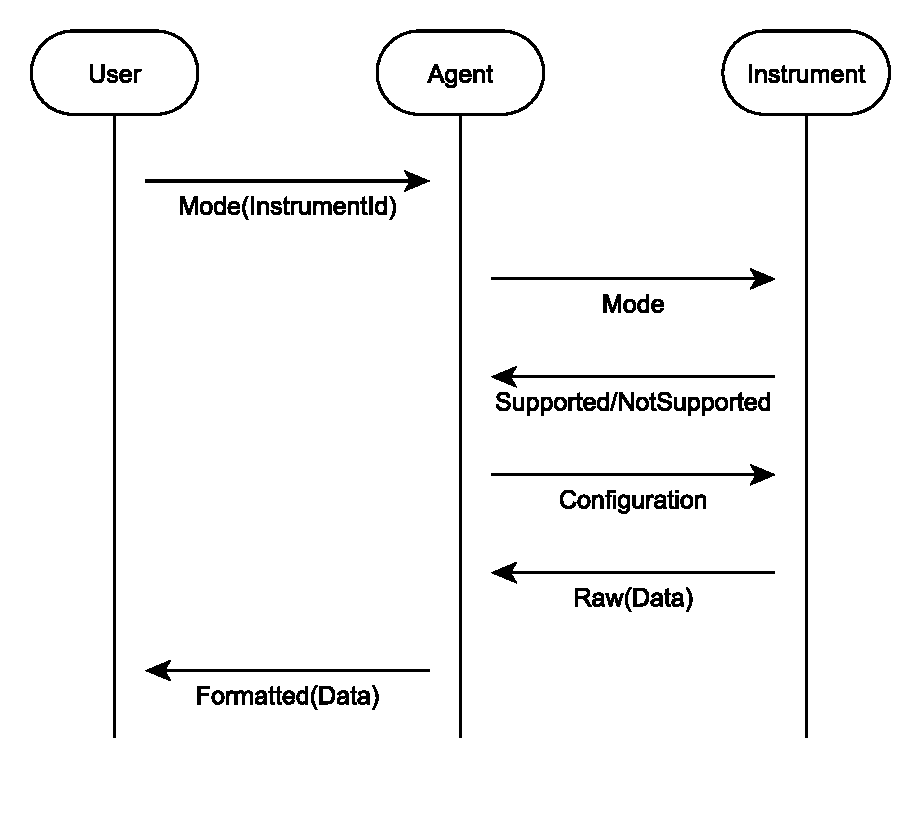
\includegraphics[width=6.5cm]{ooiUC} ~~
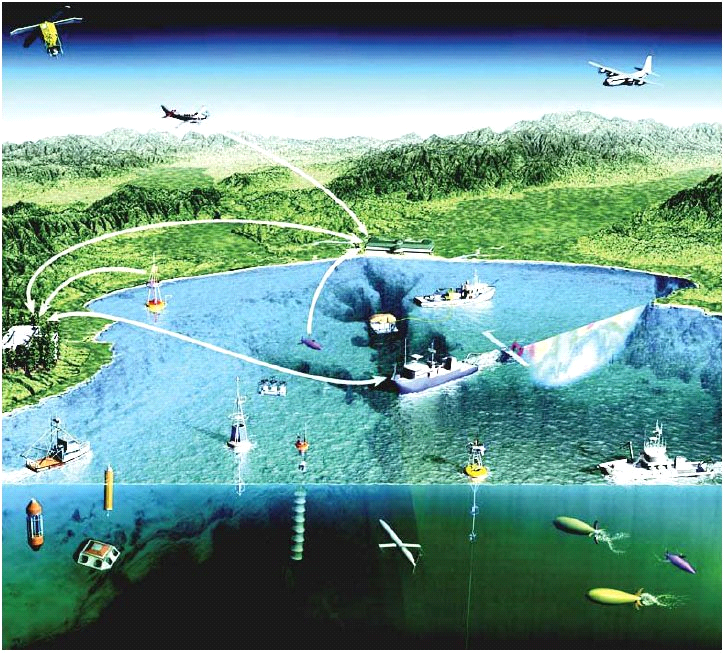
\includegraphics[width=5cm]{OOI-UseCase2}
\end{frame}

\begin{frame}{Global Protocol in SCRIBBLE}
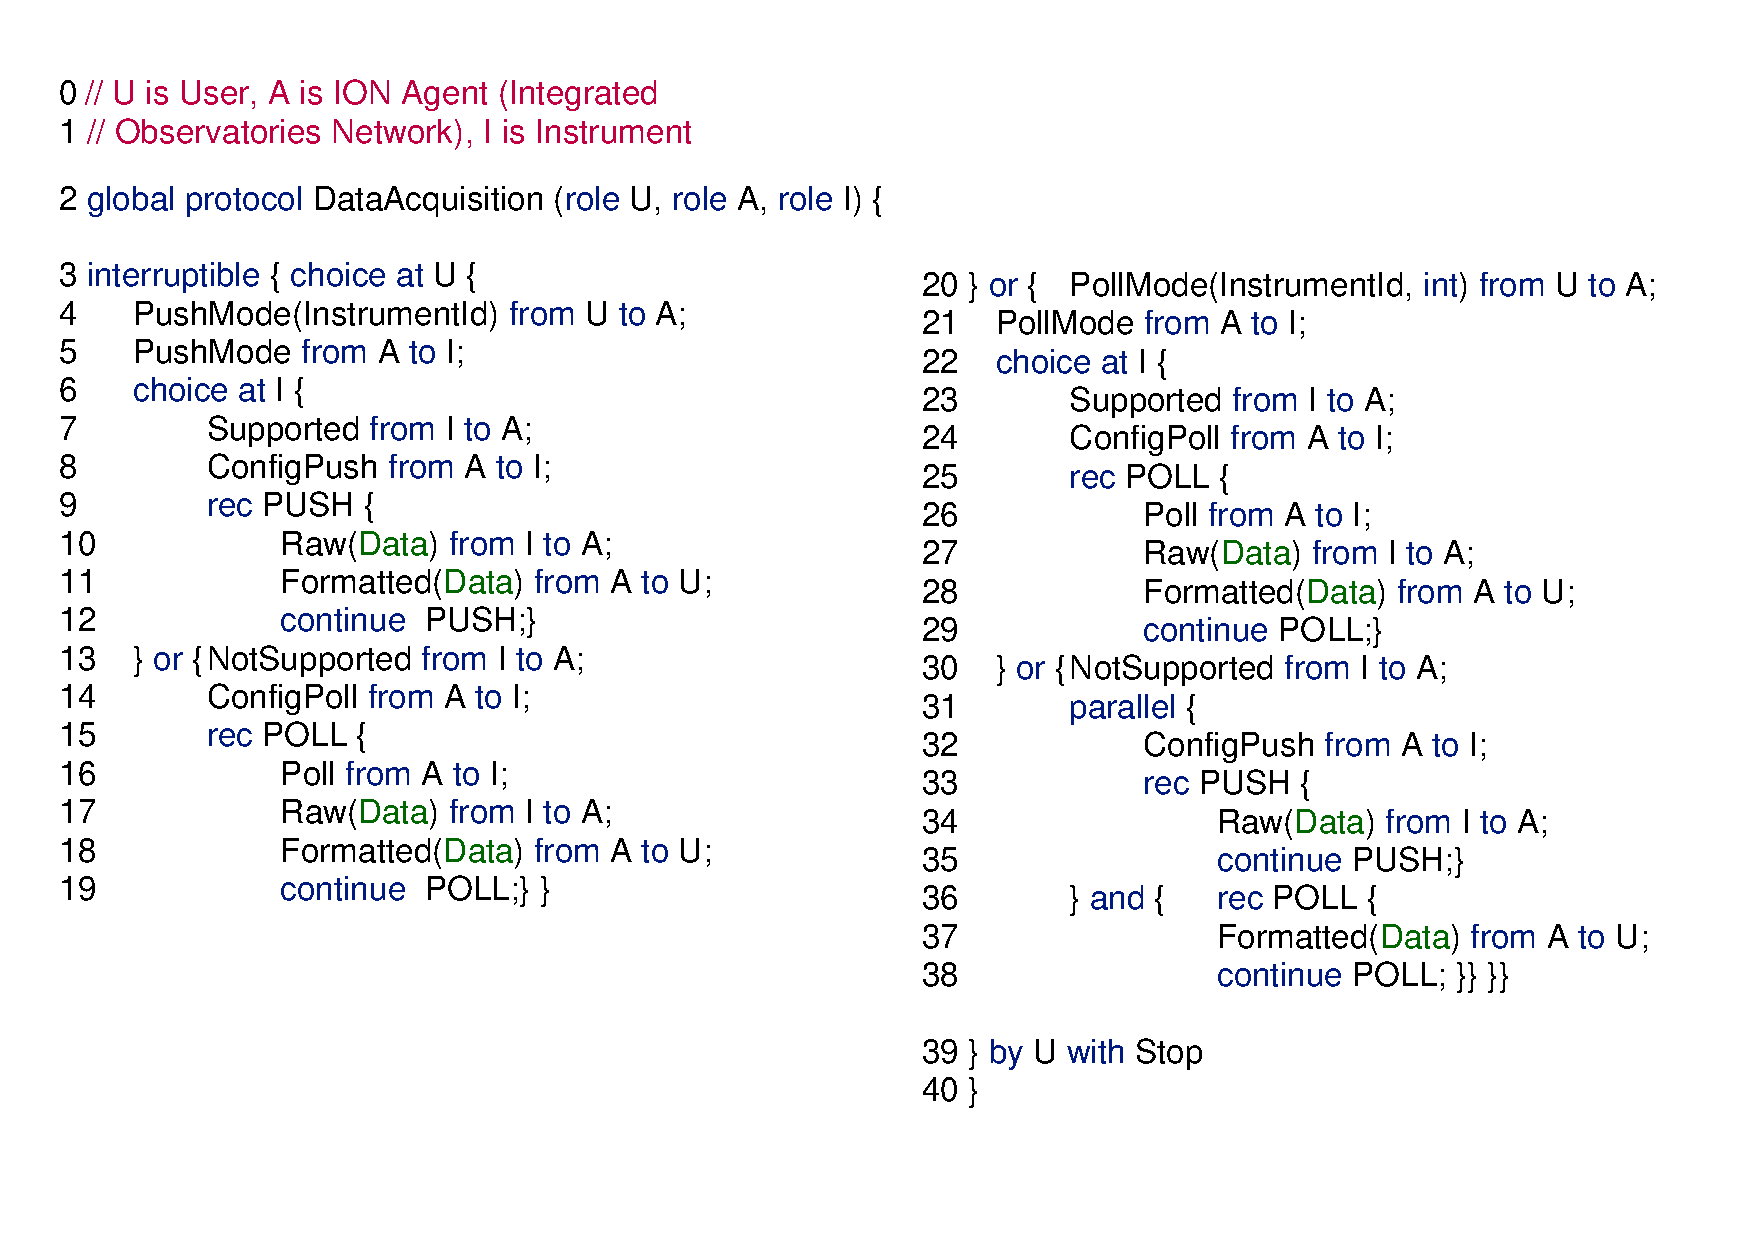
\includegraphics[width=11cm]{global-protocol}
\end{frame}

\begin{frame}{Graphical Representation}
\begin{center}
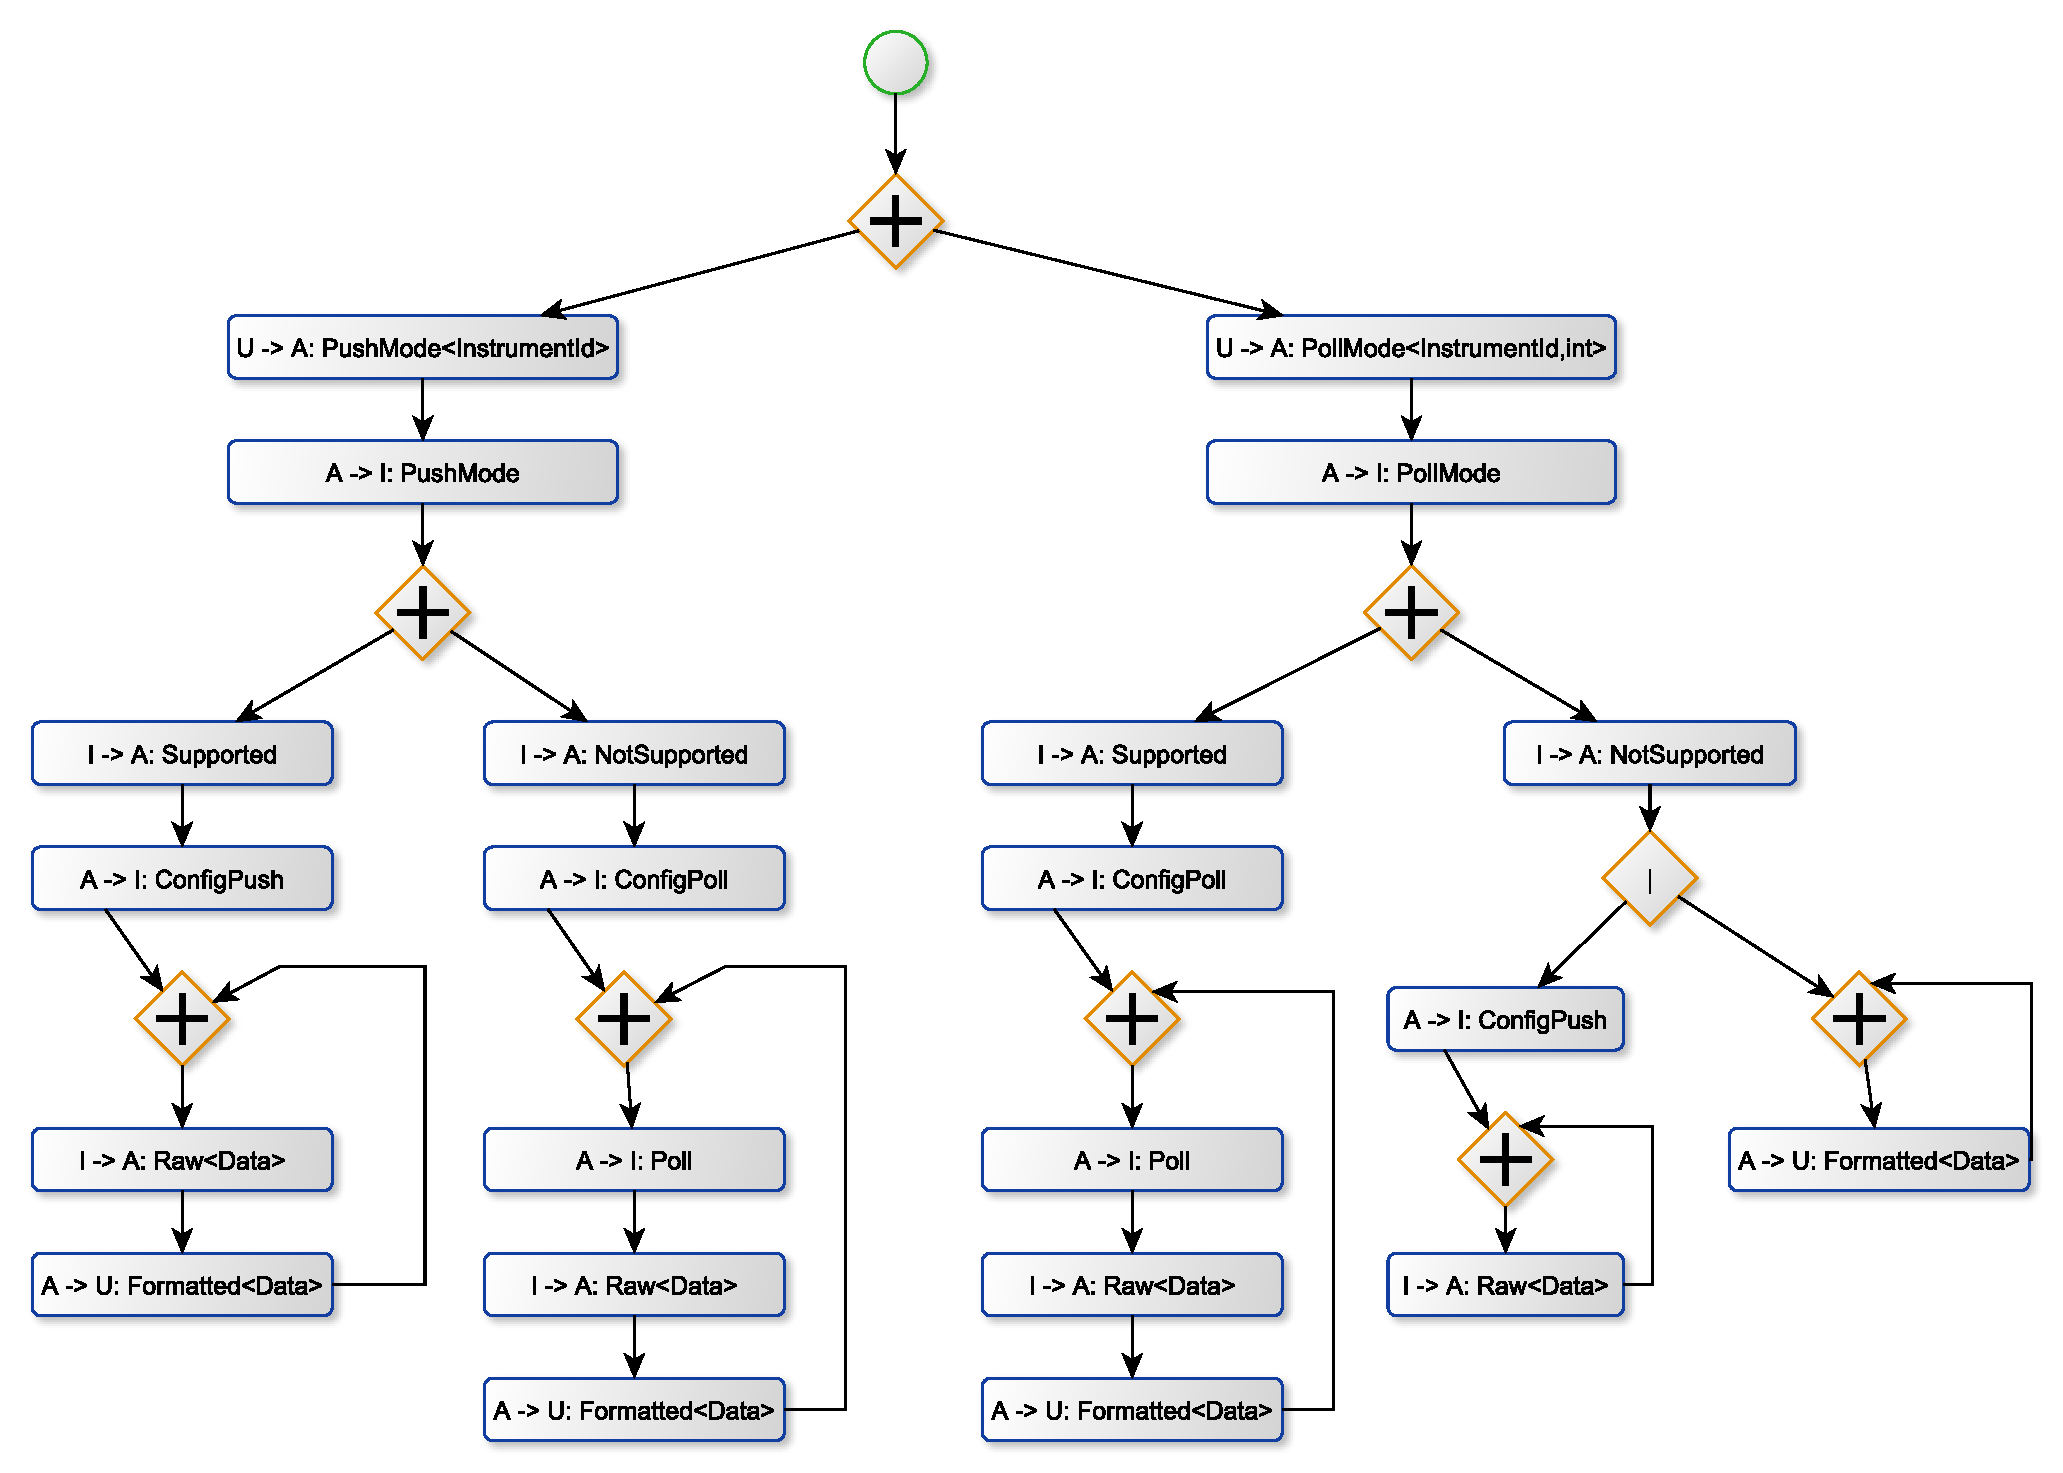
\includegraphics[height=7cm]{ooi_graph}
\end{center}
\end{frame}

\subsection{Generalised Multiparty Session Types}
\begin{frame}{Generalised Multiparty Session Types: Global Types}
\begin{center}
\begin{tabular}{rcll}
G & ::= & def $\G$ in x & Global type \\
$\G$ & ::= & x  = p $\rightarrow q : l \langle \UT \rangle;x' $ & Labelled messages\\
& | & x = x' | x'' & Fork\\
& | & x = x' + x'' & Choice\\
& | & x | x' = x'' & Join\\
& | & x + x' = x'' & Merge\\
& | & x = $\End$ & End\\
\UT & ::= &$ \langle G\rangle\ |\ \Bool\ |\ nat \ |\ \ldots\ $ & Sorts\\
\end{tabular}
\end{center}
\begin{block}{}
\begin{tabular}{rcrcl}
G =&def& $x_{0}$ &=& $x_{push} + x_{poll}$\\
&& $x_{push}$ &=& U $\rightarrow$ A: PushMode$\langle$ InstrumentId $\rangle ; x_{push1}$\\
&& $x_{push1}$ &=& A $\rightarrow$ I: PushMode ;$ x_{push2}$\\
&& $x_{push2}$ &=& $ x_{ps} + x_{pns}$\\
&& $x_{ps}$ &=& I $\rightarrow$ A: Supported$ ; x_{ps1}$\\
&& $x_{ps1}$ &=& A $\rightarrow$ I: ConfigPush$ ; x_{ps2}$\\
&& $x_{ps2} + x_{ps3}$ &=& $x_{ps4}$\\
&& $x_{ps4}$ &=& I $\rightarrow$ A: Raw$\langle$ Data $\rangle ; x_{ps5}$\\
&& $x_{ps5}$ &=& A $\rightarrow$ U: Formatted$\langle$ Data $\rangle ; x_{ps3}$\\
&& $x_{pns}$ &=& I $\rightarrow$ A: NotSupported$ ; x_{pns1}$\\
&& $x_{pns1}$ &=& A $\rightarrow$ I: ConfigPoll$ ; x_{pns2}$ ...\\
&in $x_{0}$&&&\\
\end{tabular}
\end{block}
\end{frame}

\begin{frame}{Generalised Multiparty Session Types: Graph syntax}
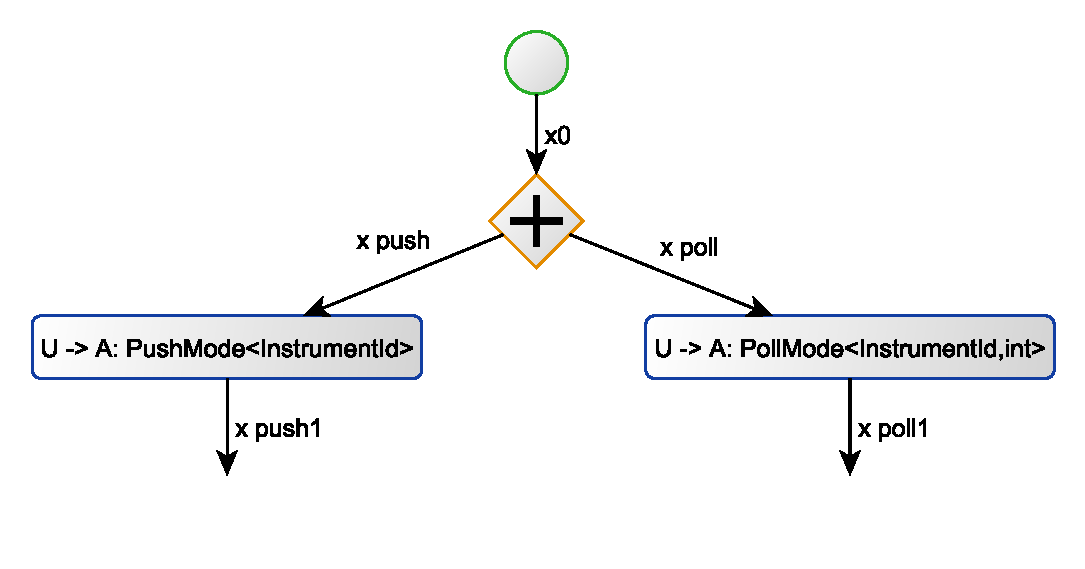
\includegraphics[scale=0.55]{ooi_graph_details}
\begin{columns}
\begin{column}<1->[b]{5cm}
\begin{exampleblock}<1->{}
{\BLUE choice at} U \{ \\
~~	PushMode(InstrumentId) {\BLUE from} U {\BLUE to} A;\\
\} {\BLUE or} \{ \\
~~	PollMode(InstrumentId,int) {\BLUE from} U {\BLUE to} A;\\
\}
\end{exampleblock}
\end{column}
\begin{column}<1->[b]{6.5cm}
\begin{block}<1->{}
\begin{tabular}{rcl}
$x_{0}$ &=& $x_{push} + x_{poll}$\\
$x_{push}$ &=& U $\rightarrow$ A: PushMode$\langle$ InstrumentId $\rangle ; x_{push1}$\\
$x_{poll}$ &=& U $\rightarrow$ A: PollMode$\langle$ InstrumentId,int $\rangle ; x_{poll1}$\\
\end{tabular}
\end{block}
~~\\
\end{column}
\end{columns}
\end{frame}

\subsection{Overview of the project}

\begin{frame}{Overview of the project}
\begin{center}
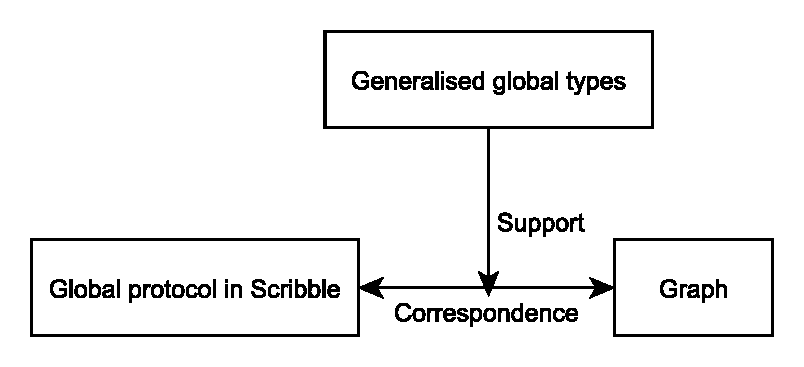
\includegraphics[width=9cm]{architecture2}
\end{center}
\end{frame}

\begin{frame}{Graphical Representation with time constraints}
\begin{center}
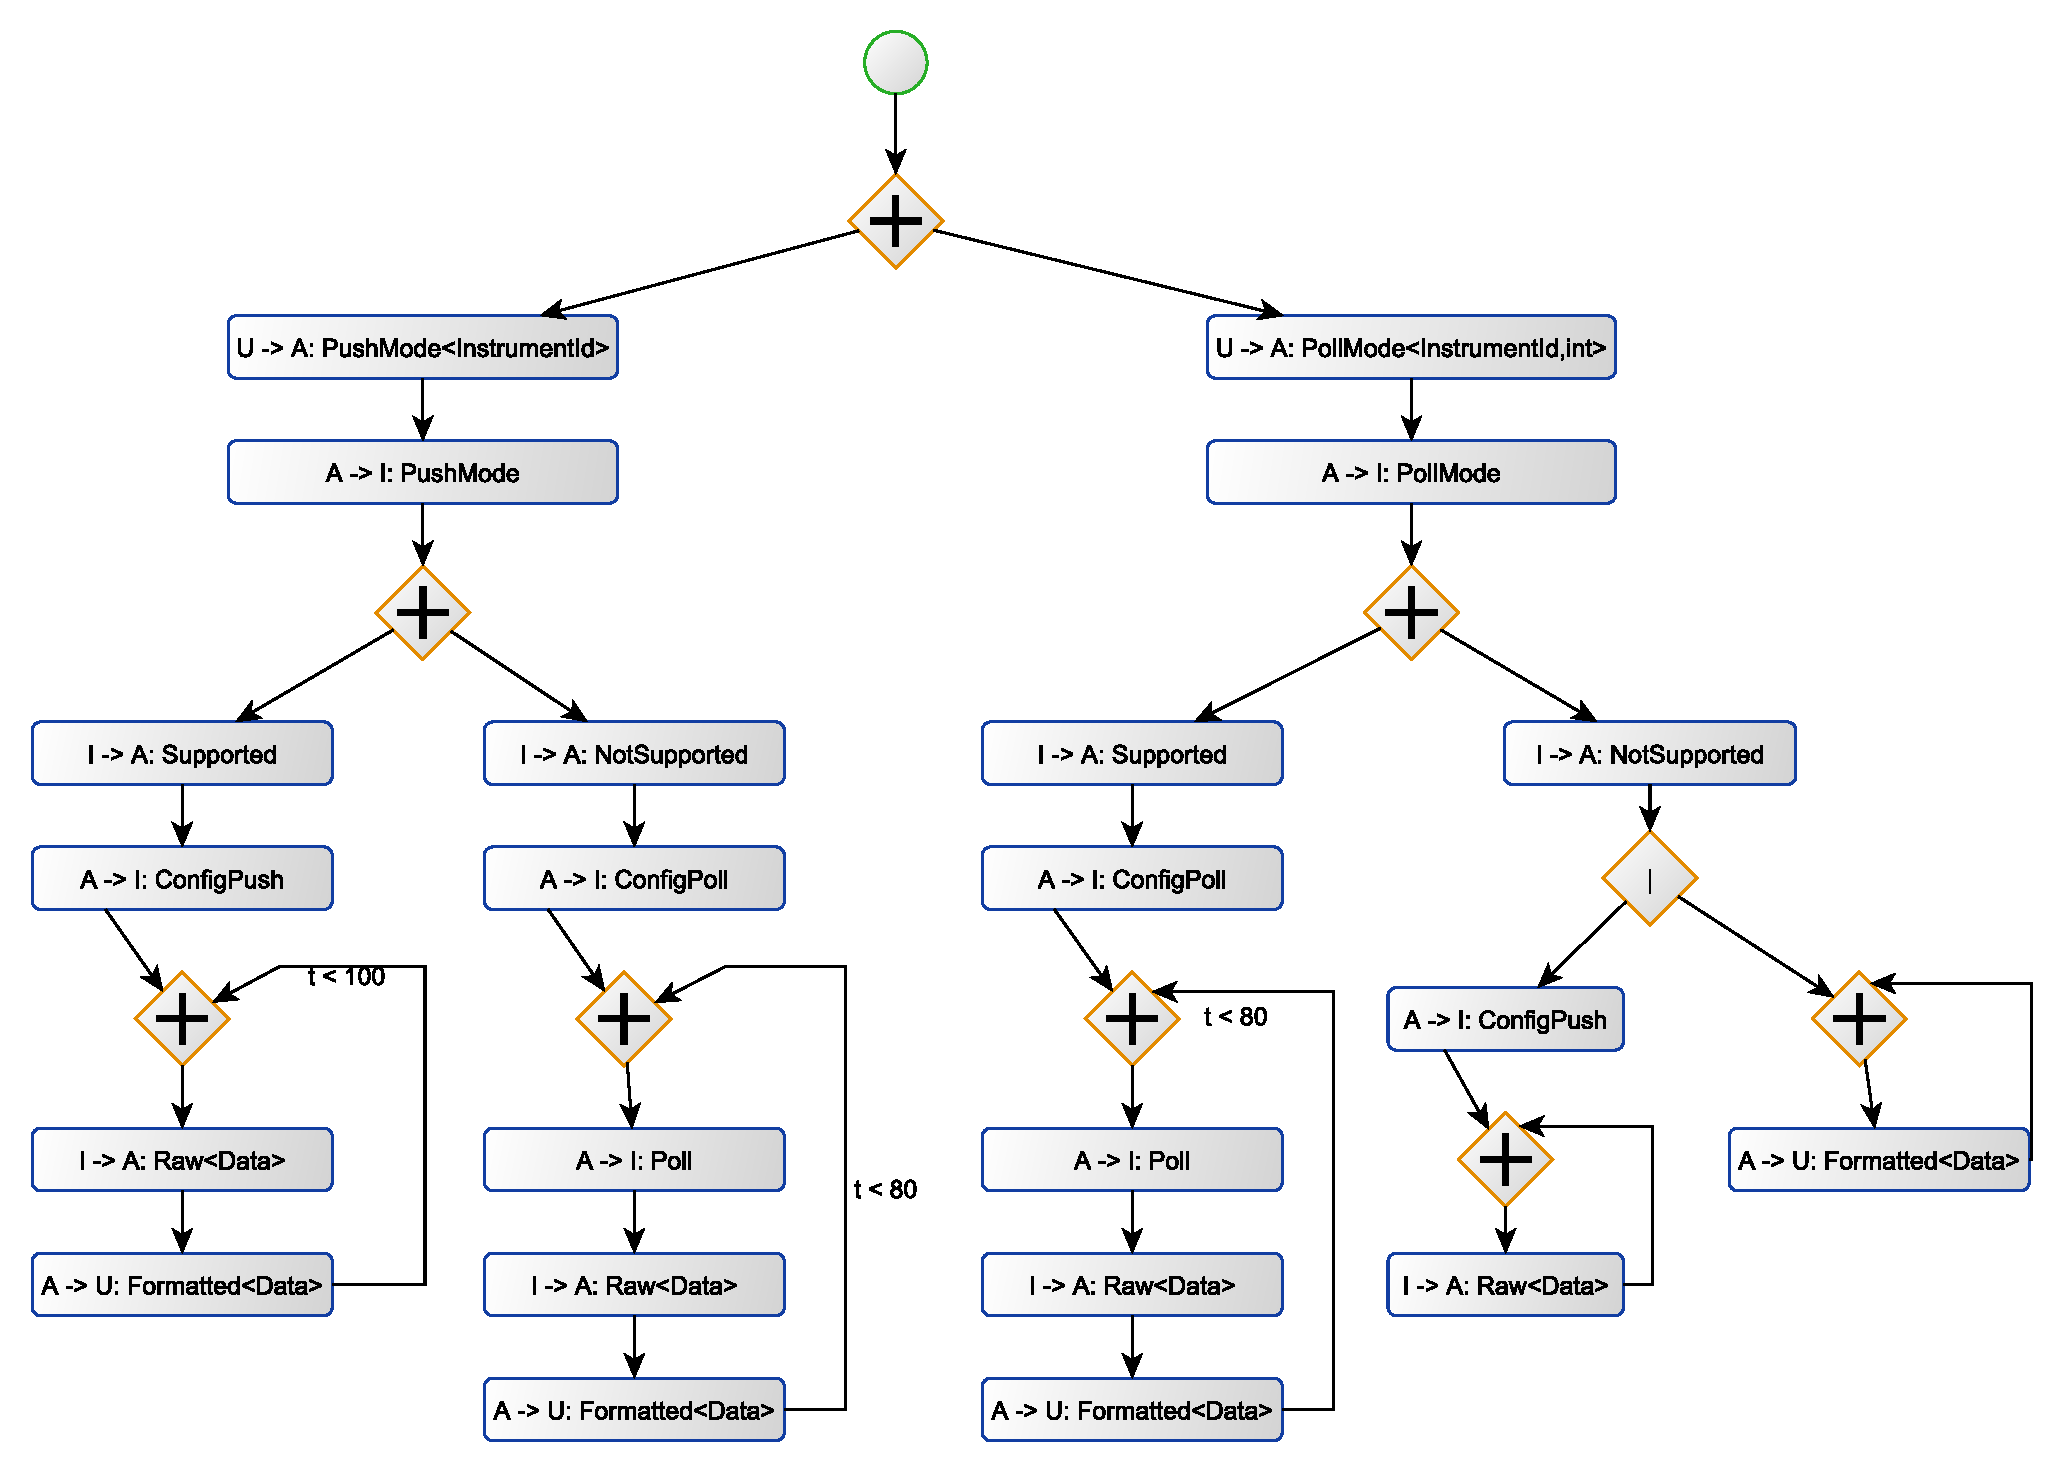
\includegraphics[height=7cm]{ooi_graph2}
\end{center}
\end{frame}

\begin{frame}{Overview of the project}
\begin{center}
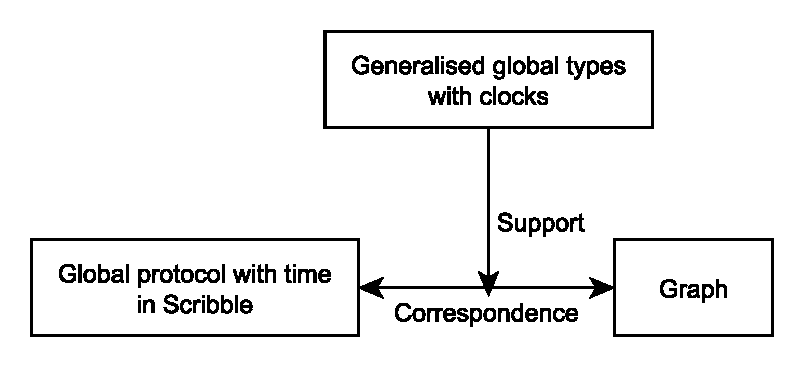
\includegraphics[width=9cm]{architecture3}
\end{center}
\pause
Contributions:
\begin{itemize}
\item<2-> Design of the graph
\item<2-> Extension with clocks
\item<2-> Implementation of the correspondence
\end{itemize}
\end{frame}

\begin{frame}{Overview of the implementation}
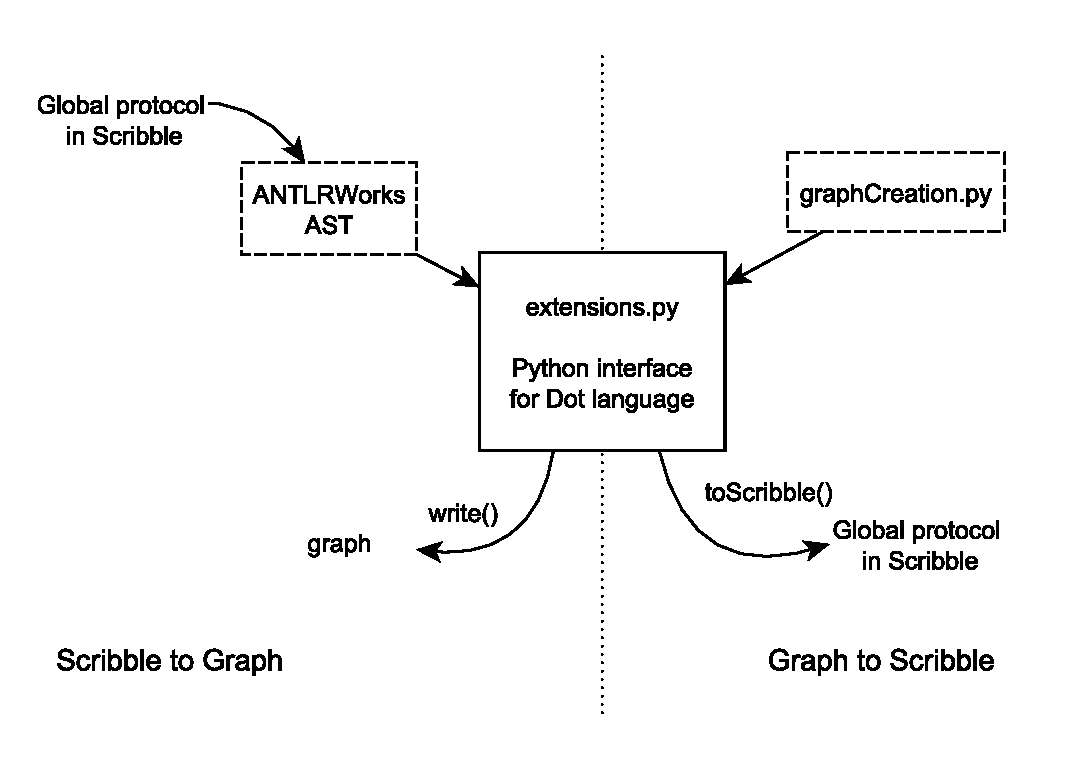
\includegraphics[scale=0.6]{structure}
\end{frame}

\section{Graph Representation}
\subsection{The design}

\begin{frame}{Graphical notations}
\begin{columns}
\begin{column}<1->[t]{5cm}
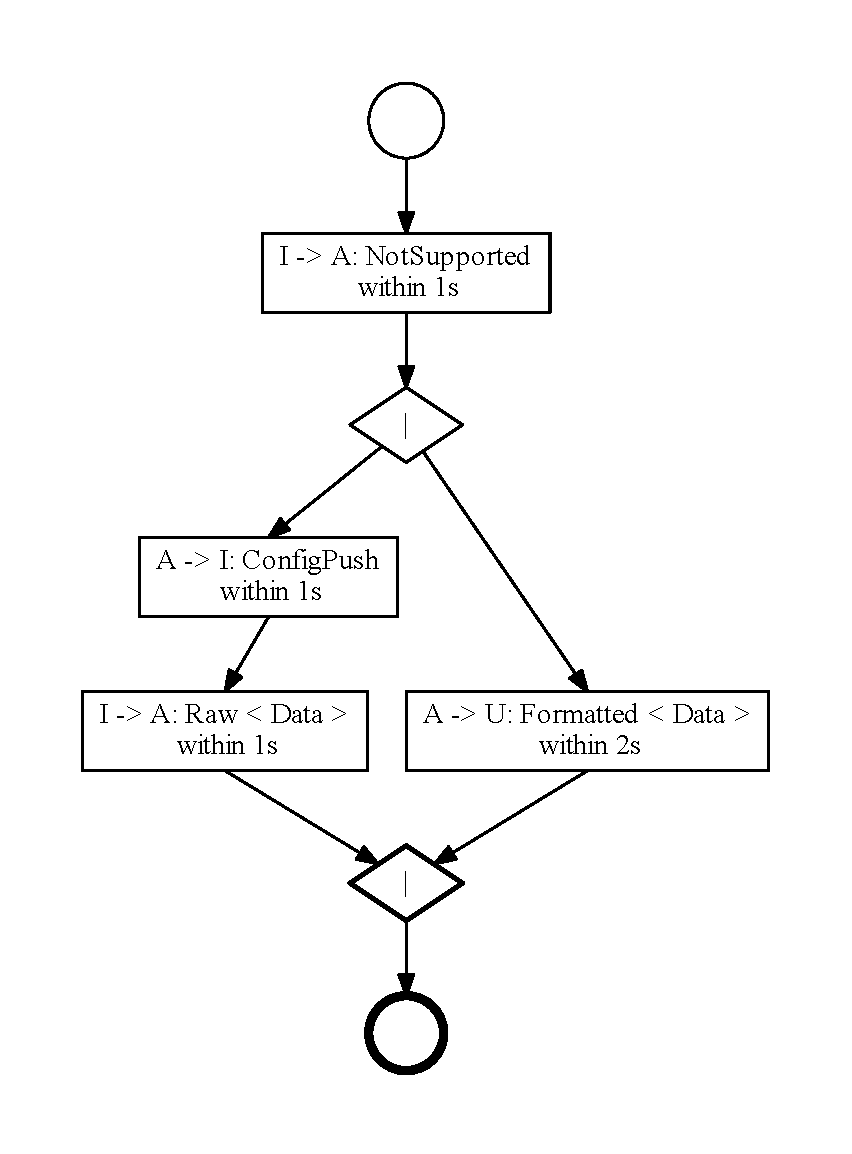
\includegraphics[height=6cm]{Parallel}
\end{column}
\begin{column}<1->[b]{6cm}
\begin{exampleblock}<1->{}
{\BLUE global protocol} FirstParallel (role U, role A, role I) \{ \\
~~NotSupported {\BLUE from} I {\BLUE to} A {\BLUE within} 1s;\\
~~parallel \{ \\
 ~~~~~~ConfigPush {\BLUE from} A {\BLUE to} I {\BLUE within} 1s;\\
 ~~~~~~Raw(Data) {\BLUE from} A {\BLUE to} I {\BLUE within} 1s;\\
~~\} and \{\\	
 ~~~~~~Formatted(Data) {\BLUE from} A {\BLUE to} U {\BLUE within} 2s;\\
~~~~~~\}\\
\}\\
\end{exampleblock}
~~\\
~~\\
~~\\
~~\\
\end{column}
\end{columns}
\end{frame}

%\begin{frame}{Graph notations}
%\begin{center}
%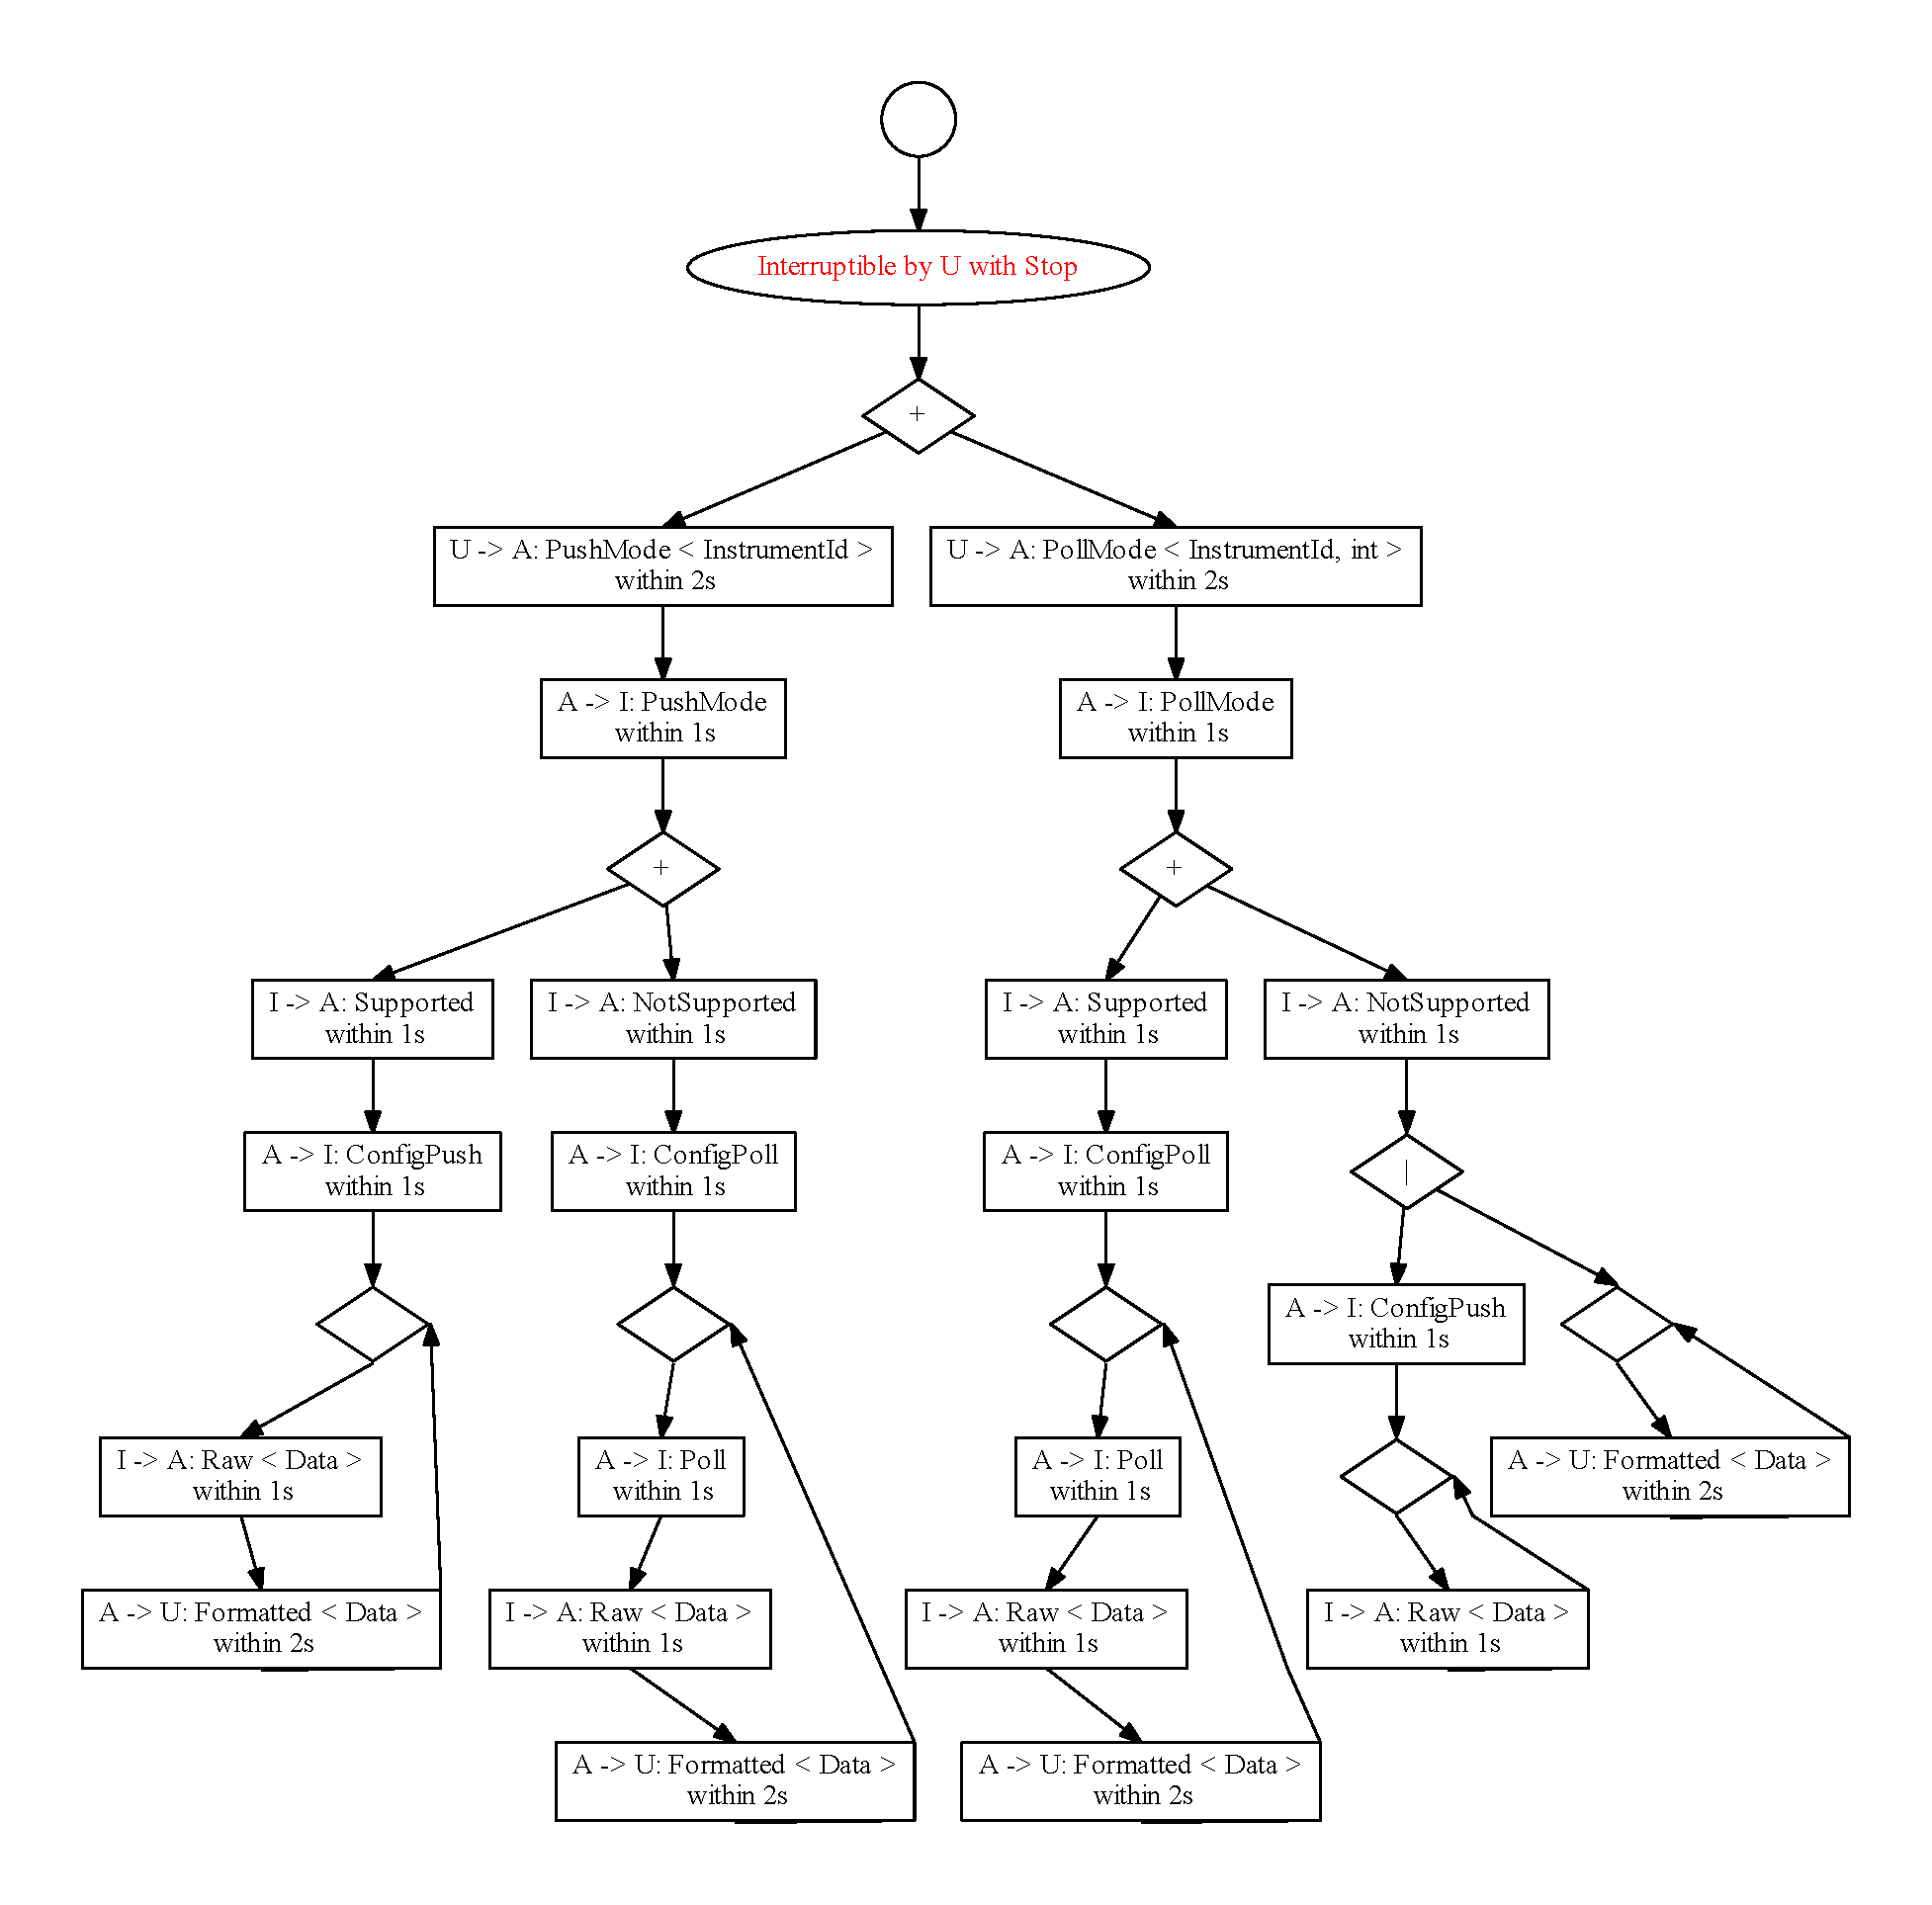
\includegraphics[height=7cm]{DataAcquisition2}
%\end{center}
%\end{frame}


\begin{frame}{Graph with clocks}
\begin{columns}
\begin{column}<1->[t]{6.5cm}
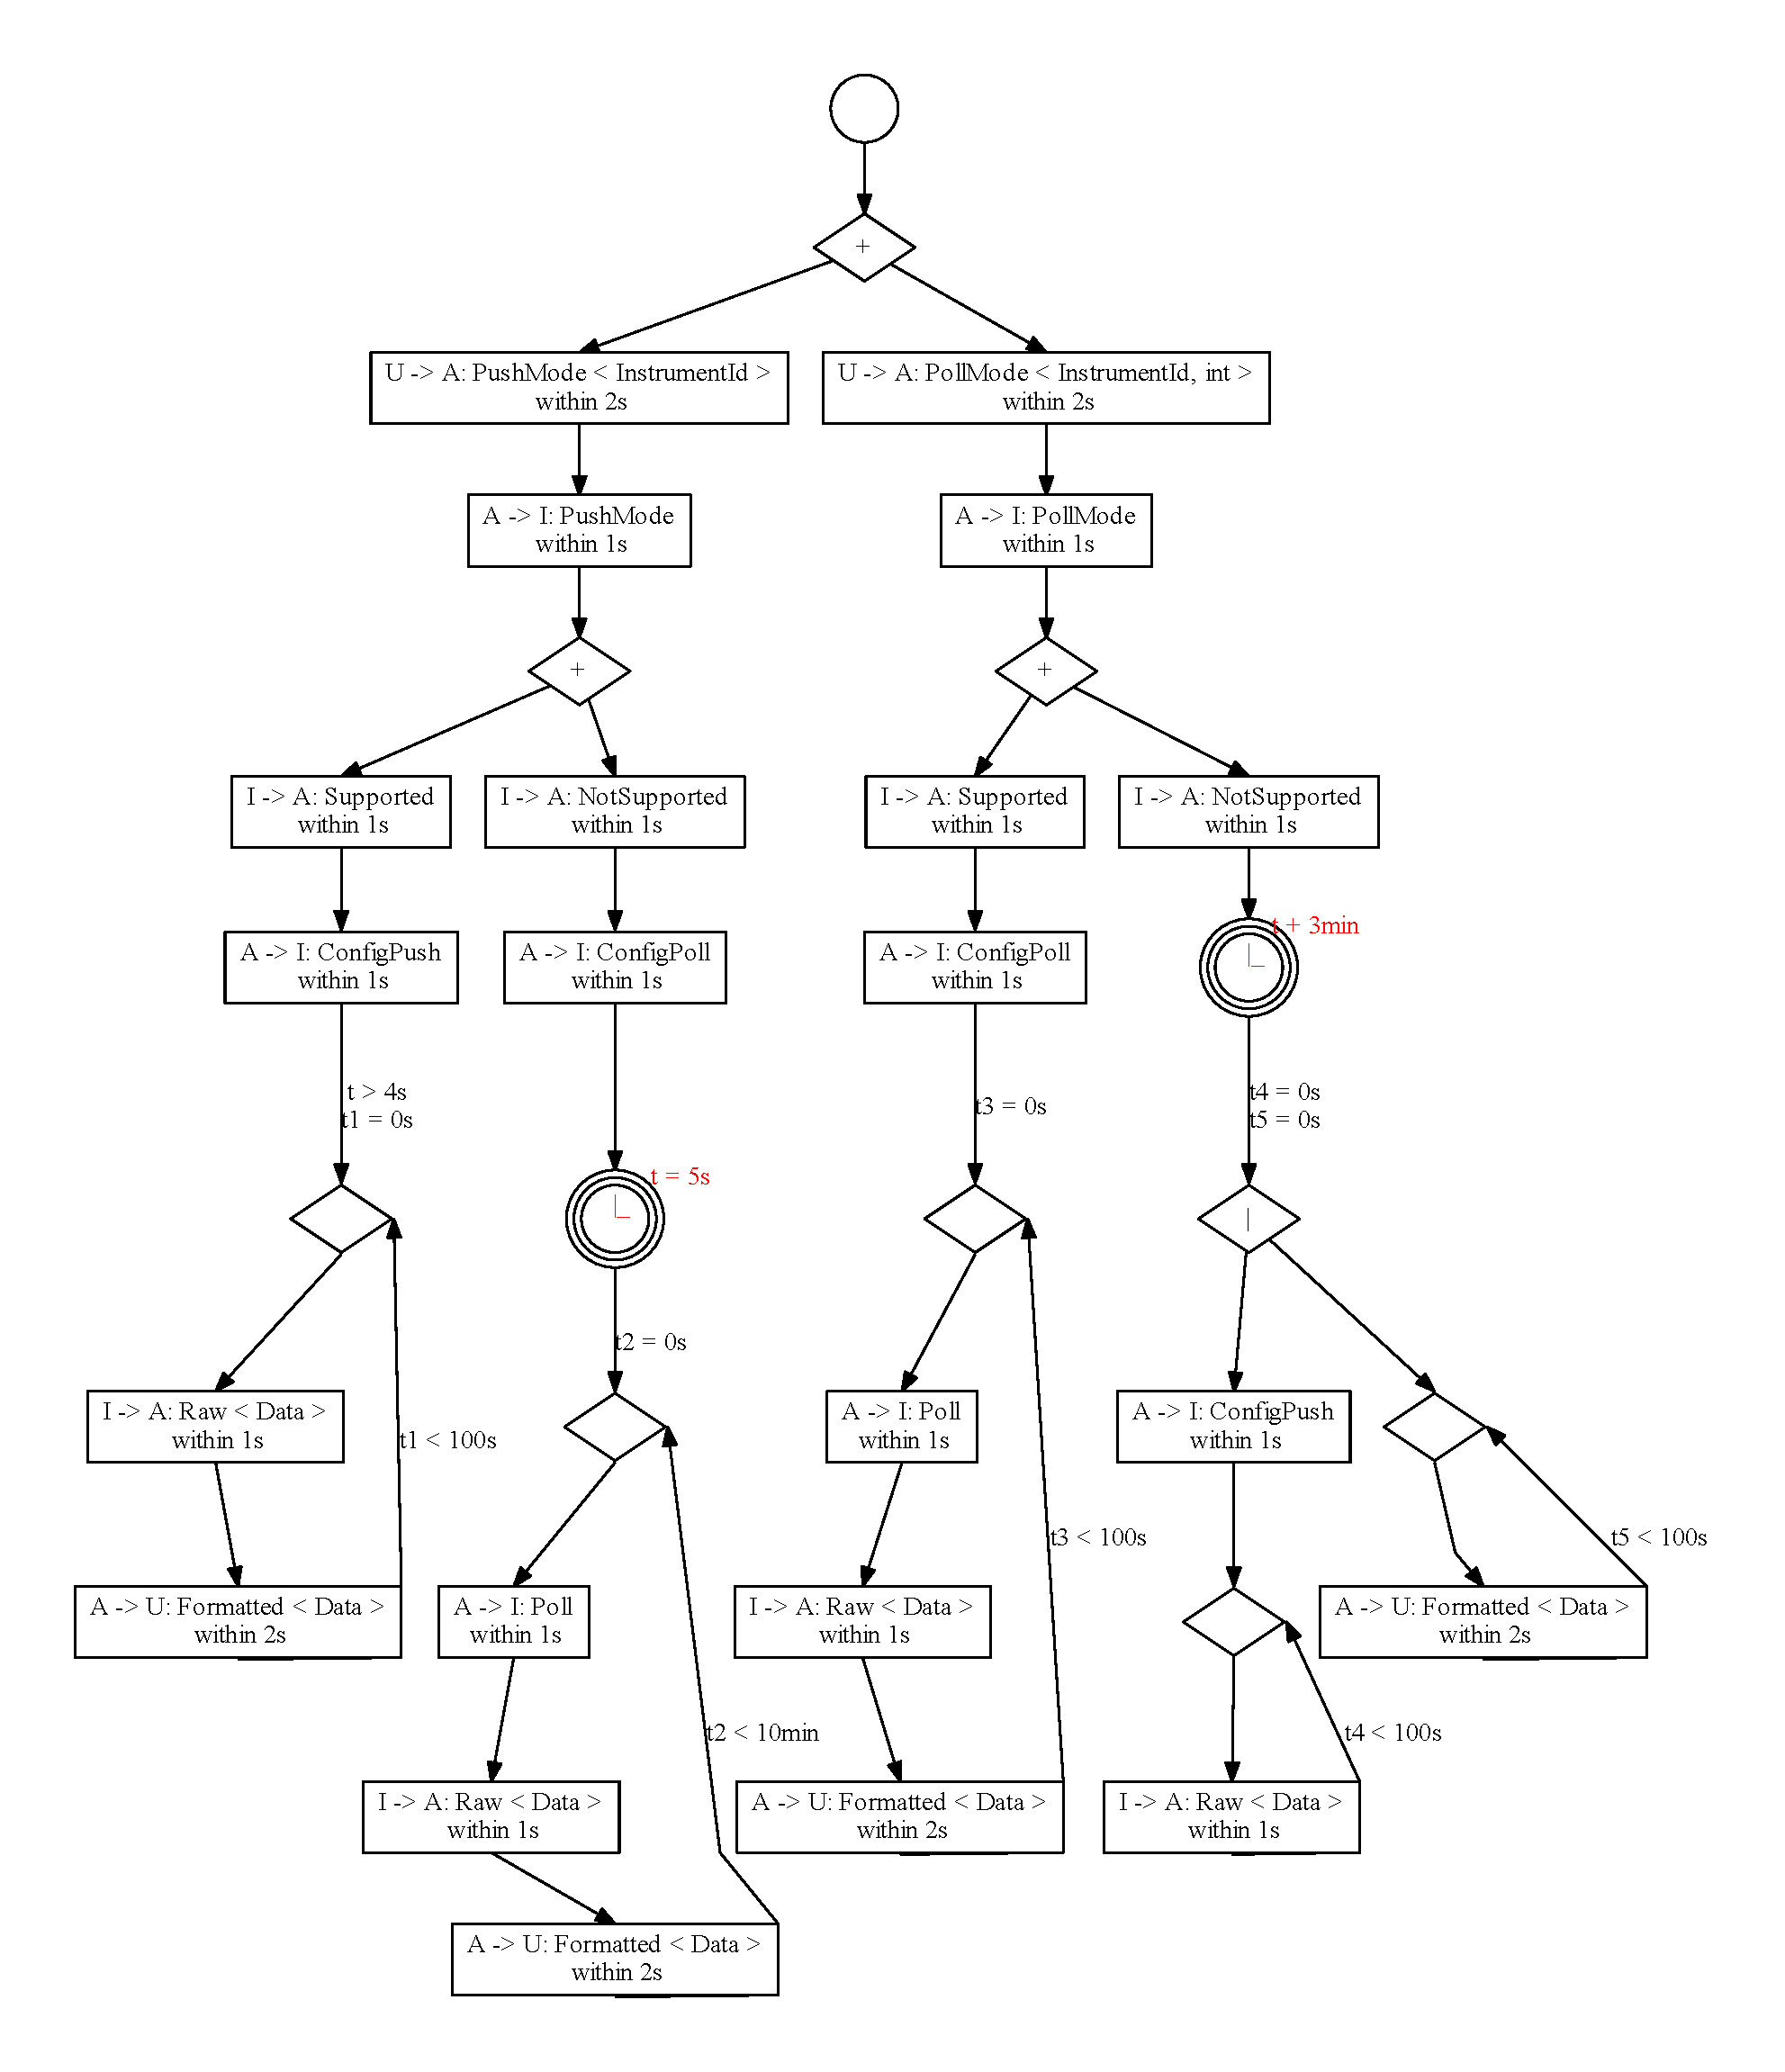
\includegraphics[height=8cm]{DataAcquisitionExample}
\end{column}
\begin{column}<1->[b]{5.5cm}

\fbox{
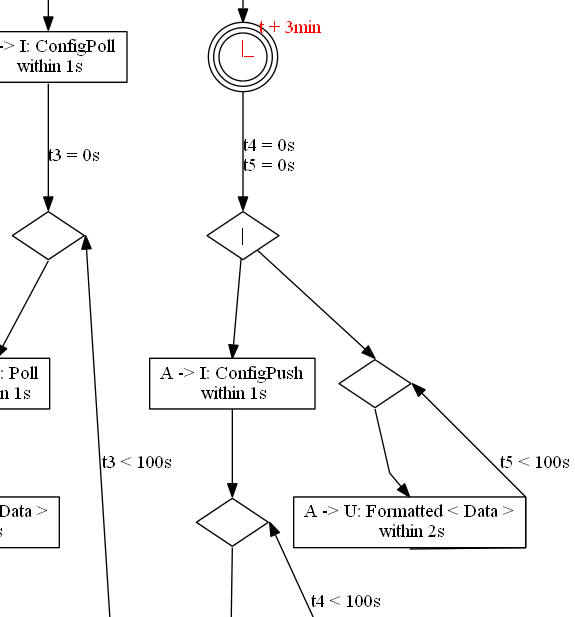
\includegraphics[width=5.5cm]{zoomDAE}
}
\\
\begin{center}
Zoom
\end{center}
~~\\~~\\~~\\
\end{column}
\end{columns}
\end{frame}


\subsection{Syntax}
\begin{frame}{Timed global types}
Let C be a set of clocks. C = \{$t, t_1, t_2, ..., t_x, ...$\}
\begin{block}<1->{Definition:}
$\delta := t \le v ~|~ t \ge v ~|~ \neg \delta ~|~ \delta_{1} \wedge \delta_{2} ~|~ \epsilon$ \\
where t is a clock in C and v is a constant in $\mathbb{Q}$.
\end{block}
\begin{block}<1->{Abbreviations:}
\begin{tabular}{rcl}
t = v& means& t $\le$ v and  t $\ge$ v\\
t < v& means& $\neg$ t $\ge$ v\\
t > v& means& $\neg$ t $\le$ v\\
\end{tabular}
\end{block}
\begin{center}
\begin{tabular}{rcll}
G & ::= & def $\tilde{\G}$ in x & Global type \\
$\G$ & ::= & x  = p $\rightarrow p' : l \langle \UT \rangle, \lambda_{O}, \delta_{O}, \lambda_{I}, \delta_{I} ;x' $ & Labelled messages\\
& | & x = x' | x'' & Fork\\
& | & x = x' + x'' & Choice\\
& | & x | x' = x'' & Join\\
& | & x + x' = x'' & Merge\\
& | & x = $\End$ & End\\
\UT & ::= &$ \langle G\rangle\ |\ \Bool\ |\ nat \ |\ \ldots\ $ & Sorts
\end{tabular}
\end{center}
\end{frame}

\begin{frame}{Timed local types and projection}
\begin{center}
\begin{tabular}{rcll}
T & ::= & def $\tilde{\T}$ in x & Local type \\
$\T$ & ::= & x  = !$\langle p,  l \langle \UT \rangle, \lambda, \delta \rangle.x' $ & Message sending\\
& | & x  = ?$\langle p,  l \langle \UT \rangle, \lambda, \delta \rangle.x' $ & Message receiving\\
& | & x = x' | x'' & Fork\\
& | & x = x' $\oplus$ x'' & Internal choice\\ 
& | & x = x' \& x'' & External choice\\
& | & x | x' = x'' & Join\\
& | & x + x' = x'' & Merge\\
& | & x = x' & Inaction\\
& | & x = $\End$ & End\\
\end{tabular}
\end{center}
Projection algorithm:\\
\begin{tabular}{rcll}
def $\tilde{\G}$ in x $\upharpoonright$ p & = & def $\tilde{\G}\upharpoonright_{\tilde{\G}}$ p in x &\\
&&&\\
x  = p $\rightarrow p' : l \langle \UT \rangle, \lambda_{O}, \delta_{O}, \lambda_{I}, \delta_{I} ;x' \upharpoonright_{\tilde{\G}}$ p & = &  x  = !$\langle p',  l \langle \UT \rangle, \lambda_{O}, \delta_{O} \rangle.x' $ &\\
x  = p $\rightarrow p' : l \langle \UT \rangle, \lambda_{O}, \delta_{O}, \lambda_{I}, \delta_{I} ;x' \upharpoonright_{\tilde{\G}}$ p' & = &  x  = ?$\langle p,  l \langle \UT \rangle, \lambda_{I}, \delta_{I} \rangle.x' $ &\\
x  = p $\rightarrow p' : l \langle \UT \rangle, \lambda_{O}, \delta_{O}, \lambda_{I}, \delta_{I} ;x' \upharpoonright_{\tilde{\G}}$ p'' & = &  x = x' &(p'' $\notin$ \{p,p'\})\\
x = x' | x'' $\upharpoonright_{\tilde{\G}}$ p & = &  x = x' | x''&\\
x = x' + x'' $\upharpoonright_{\tilde{\G}}$ p & = & x = x' $\oplus$ x'' &(if p = ASend($\tilde{\G}$)(x))\\
x = x' + x'' $\upharpoonright_{\tilde{\G}}$ p & = & x = x' \& x'' &(otherwise)\\
x | x' = x'' $\upharpoonright_{\tilde{\G}}$ p & = &  x | x' = x'' &\\
x + x' = x'' $\upharpoonright_{\tilde{\G}}$ p & = & x + x' = x'' &\\
x = $\End$ $\upharpoonright_{\tilde{\G}}$ p & = & x = $\End$ &\\
\end{tabular}
\end{frame}

\begin{frame}{Timed global types: Example}
\begin{center}
x  = p $\rightarrow p' : l \langle \UT \rangle, \lambda_{O}, \delta_{O}, \lambda_{I}, \delta_{I}$ ;x'
\end{center}
\begin{center}
x = A $\rightarrow$ B : TheMessage <bool> , \{$t_{x}\}, t < 3, \{t_1\}, t_{x}$ < 2  ;  x’ 
\end{center}
\begin{columns}
\begin{column}<1->[t]{4cm}
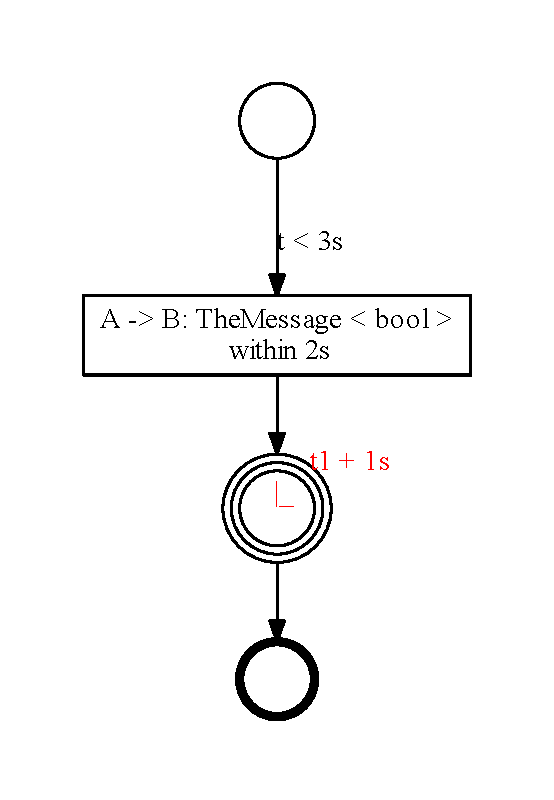
\includegraphics[height=4cm]{ExampleCFSM}
\end{column}
\begin{column}<1->[b]{5cm}
\begin{exampleblock}<1->{}
{\BLUE global protocol} Example (role A, role B) \{ \\
~~ t {\BLUE before} 3s\\
~~TheMessage(bool) {\BLUE from} A {\BLUE to} B {\BLUE within} 2s;\\
~~{\BLUE wait for} t1+ 1s\\
\}\\
~~\\
~~\\
\end{exampleblock}
\end{column}
\end{columns}
\end{frame}

\begin{frame}{The \emph{within} statement}
\begin{columns}
\begin{column}<1->[t]{5cm}
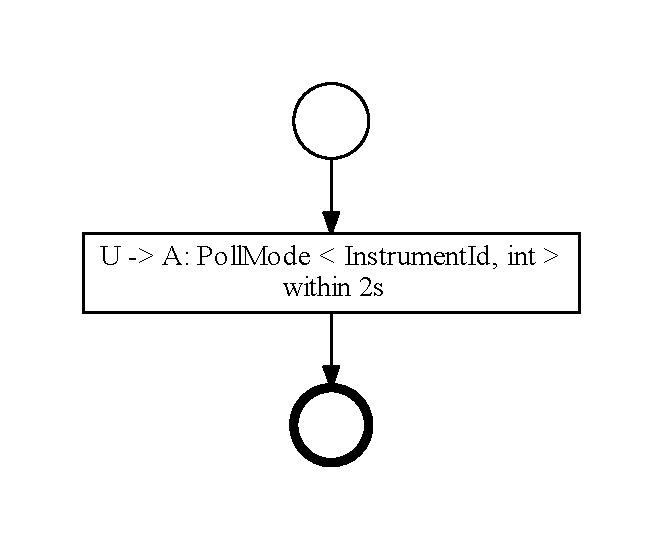
\includegraphics[height=4cm]{Message}
\end{column}
\begin{column}<1->[b]{6cm}
\begin{exampleblock}<1->{}
{\BLUE global protocol} TestMessage (role A, role U) \{ \\
~~PollMode(InstrumentId,int) {\BLUE from} U {\BLUE to} A {\BLUE within} 2s;\\
\}\\
\end{exampleblock}
~~\\
~~\\
~~\\
~~\\
~~\\
~~\\
\end{column}
\end{columns}
To support this protocol we define the global type as follows:\\
\begin{tabular}{lrl}
G = & def & x = U $\rightarrow$ A : PollMode <InstrumentId, int> , \{$t_{x}\}, \epsilon, \varnothing, t_{x}$ < 2  ;  x’\\
&& x’ = end\\
& in x&\\
\end{tabular}\\
\begin{tabular}{lrl}
$T_{U}$ = & def &  x  = !$\langle$ A, PollMode <InstrumentId, int>  ,\{$t_{x}\},\epsilon \rangle$ . x’\\
&& x’ = end\\
& in x&\\
\end{tabular}\\
\begin{tabular}{lrl}
$T_{A}$ = & def &  x  = ?$\langle$ U,PollMode <InstrumentId, int>  , $\varnothing, t_{x} < 2 \rangle$ . x’\\
&& x’ = end\\
& in x&\\
\end{tabular}\\
\end{frame}



\subsection{Results}
\begin{frame}{Temporal satisfiability for clocks conditions}
\begin{columns}
\begin{column}<1->[b]{6cm}
\textbf{Temporal satisfiability }\textit{ If $\delta$, the clock condition of a given transition, is satisfiable at some point, for each constraint $\delta$', appearing in a later transition, it is eventually possible to satisfy $\delta$'.}\\
~~\\
~~\\
\begin{exampleblock}<1->{}
{\BLUE global protocol} TestTemporalSatisfiability (role A, role B, role C) \{ \\
~~{\BLUE wait for} t {\BLUE is} 5s\\
~~Msg1(no1) {\BLUE from} A {\BLUE to} B {\BLUE within} 2s;\\
~~~~~~{\BLUE choice at} B \{ \\
~~~~~~~~~~t {\BLUE after} 6s\\
~~~~~~~~~~Msg2(no2) {\BLUE from} B {\BLUE to} C {\BLUE within} 1s;\\
~~~~~~\} {\BLUE or} \{ \\
~~~~~~~~~~Msg3(no3) {\BLUE from} B {\BLUE to} C {\BLUE within} 1s;\\
~~~~~~\}
\}\\
\end{exampleblock}
\end{column}
\begin{column}<1->[t]{5cm}
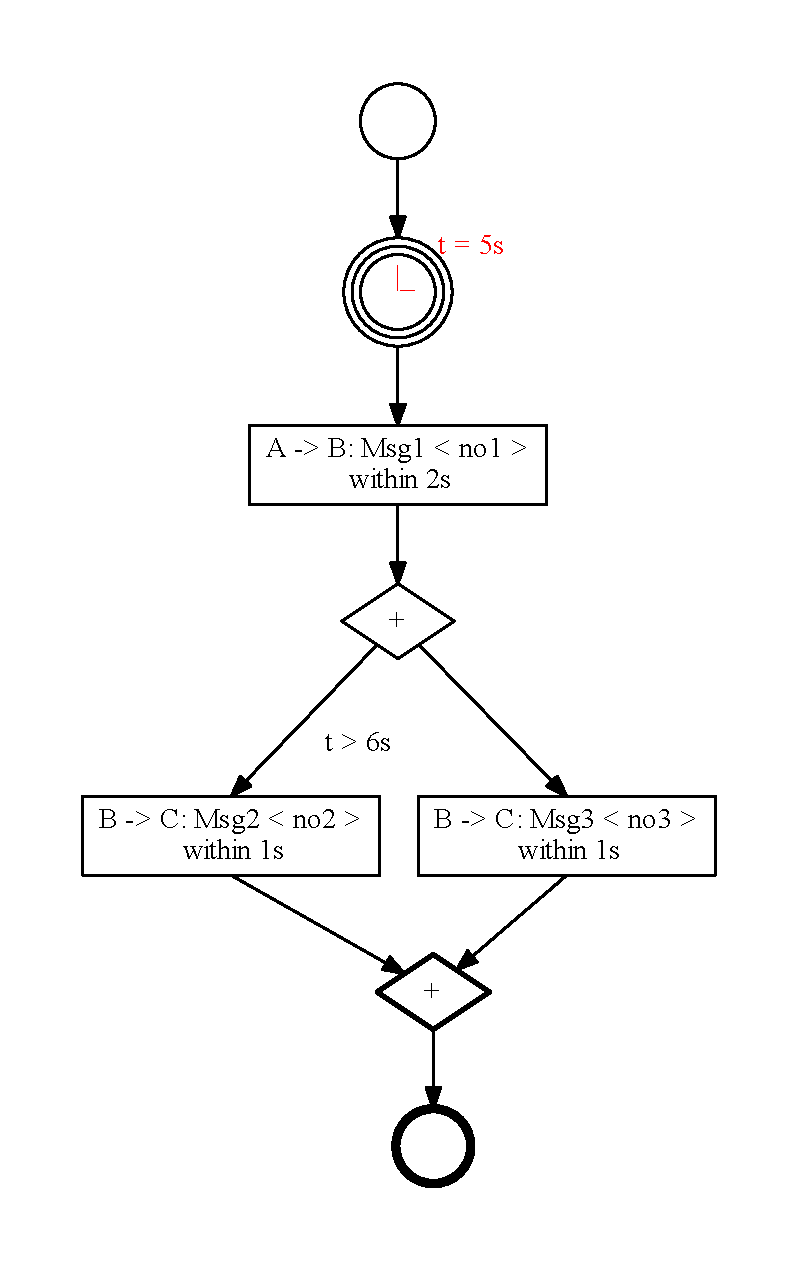
\includegraphics[height=7cm]{TestTemporalSatisfiability}
\end{column}
\end{columns}
\end{frame}

\begin{frame}{Timed processes}
\begin{table}[tb]
\centering
\begin{tabular}{rclr}
P &::= & def $\tilde{\PP}$ in X & {definition}\\
 \PP & ::=  &  x($\tilde{x}$) = x$\langle G, C \rangle$.x’($\tilde{e}$)   &   {init}\\
     & \sep & x($\tilde{x}$) = x[p](y): x’($\tilde{e}$)   &   {accept}\\
     & \sep & x($\tilde{x}$) = x!$\langle p; l<e>, \lambda_{O}, \delta_{O} \rangle$: x’($\tilde{e}$)&    {send}\\
     & \sep &  x($\tilde{x}$) = x?$\langle p; l(y), \lambda_{I}, \delta_{I} \rangle$: x’($\tilde{e}$)  &    {receive}\\
     & \sep & x($\tilde{x}$) = x’($\tilde{y}$) | x’’($\tilde{z}$)  & {parallel}\\
     & \sep & x($\tilde{x}$) | x’($\tilde{y}$) = x’’($\tilde{z}$)  &  {join}\\
     & \sep & x($\tilde{x}$)+ x’($\tilde{x}$) = x’’($\tilde{x}$)  & {merge}\\
     & \sep & x($\tilde{x}$) = x’($\tilde{x}$) \& x’’($\tilde{x}$) & {external choice}\\[1mm]
     & \sep & \ifthenelse{\e}{x'(\tilde{e}')}{x''(\tilde{e}'')} & {conditional}\\
      & \sep & x($\tilde{x}$) = 0  & {null}\\
      & \sep & x($\tilde{x}$) = \nuc{\Ia}{x’(a\tilde{x}) } & {new name}\\
X &::= &  x($\tilde{v}$) \sep  X | X & {thread, parallel} \\
 & \sep & x\nuc{\Ia}{X}  \sep 0 & {restriction, null} \\
&&&\\
\e   & ::= & v \sep x \sep e $\wedge ~\delta$ \sep e $\wedge$ e \sep $\ldots$ & {expressions}  \\
v &::= & a \sep s[p] \sep true \sep false \sep ... & {values}\\
&&&\\
$\alpha, \beta$   & ::= & s[p,q]!$\langle p; l<e>, \lambda, \delta \rangle$ &{labels}\\
 & \sep & s[p,q]?$\langle p; l(y), \lambda, \delta \rangle$ &\\
& \sep&  a$\langle G, C \rangle$ \sep a$\langle p \rangle$ [s] \sep $\langle \tau, \lambda, \delta \rangle$ & \\
\end{tabular}
\ \vspace{1mm}
\caption{Syntax for timed processes}\label{tab:timedprocesses}
\end{table}
\end{frame}



\section{About the Implementation}

\subsection{Structure of the development}
\begin{frame}{Overview}
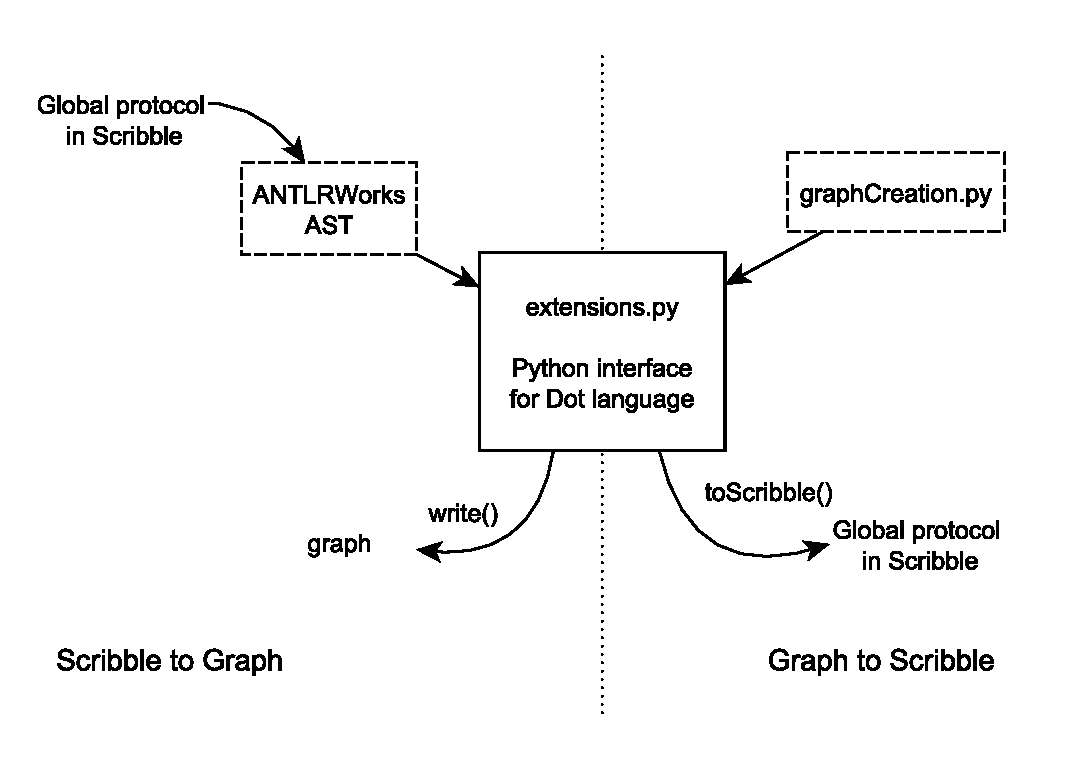
\includegraphics[scale=0.6]{structure}
\end{frame}

\begin{frame}{Link between ANTLRWorks and Eclipse}
\begin{tabular}{lr}
 &
\includegraphics[width=0.7cm]{python}\\
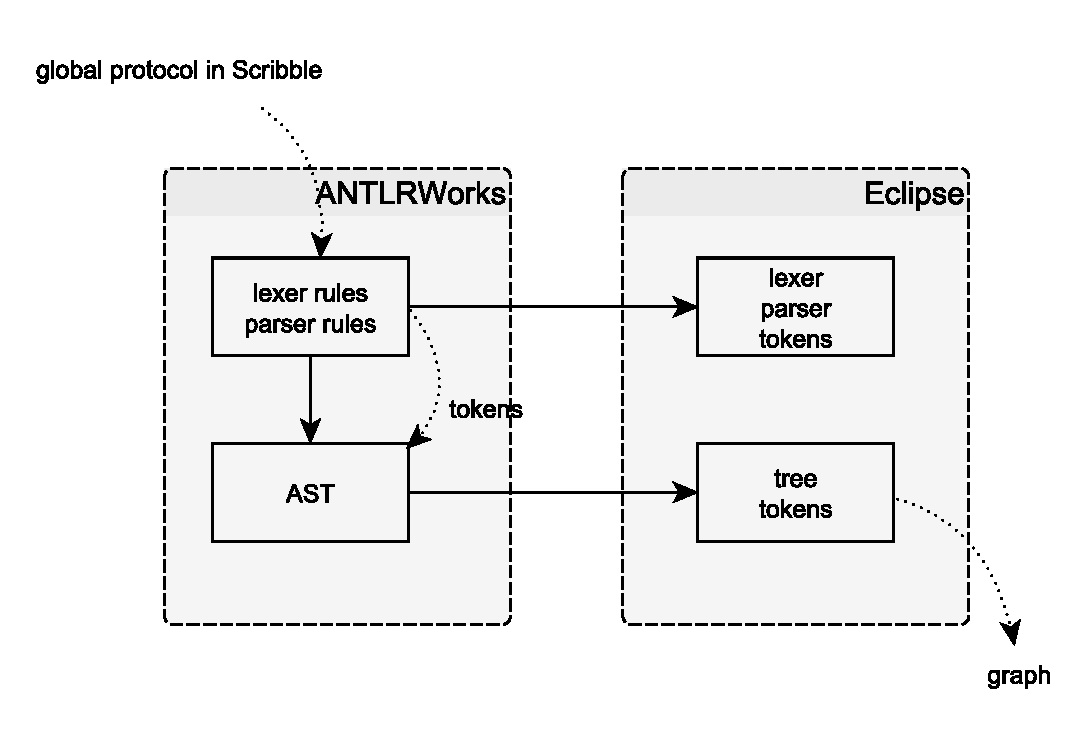
\includegraphics[scale=0.5]{zoomstructure}&\\
\end{tabular}
\end{frame}



\subsection{Demonstration}

\begin{frame}{Demonstration}
%demo
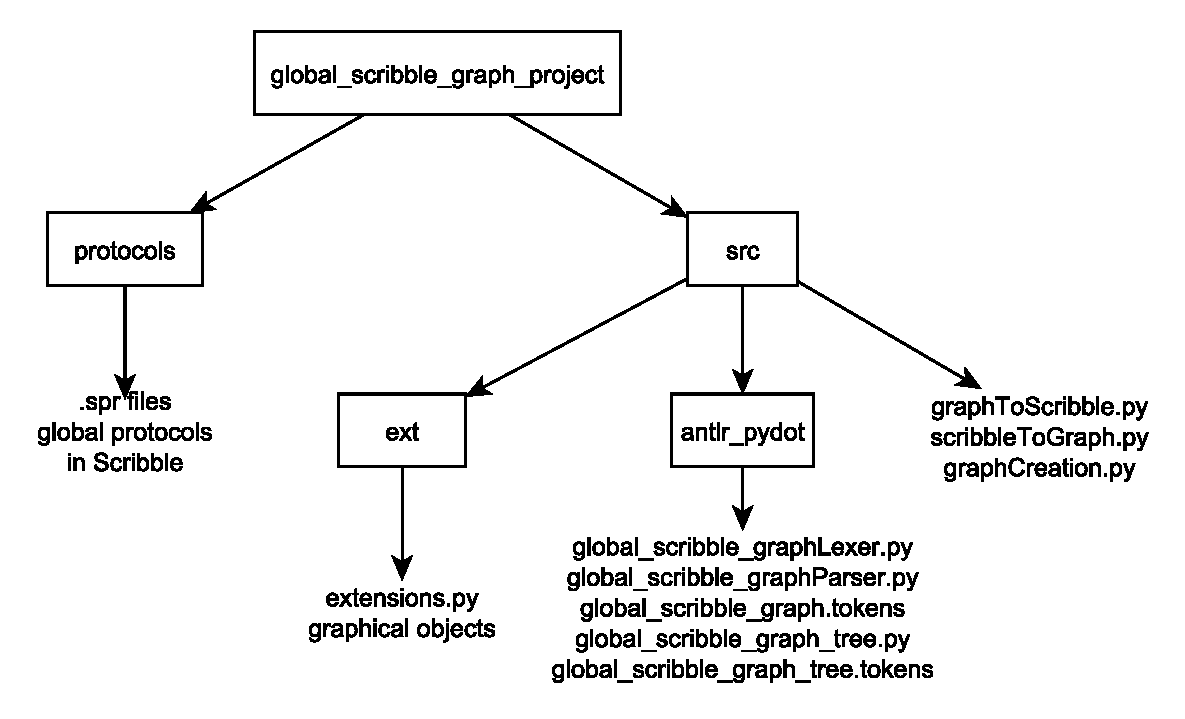
\includegraphics[width=11cm]{project_organisation}
\end{frame}

\subsection*{Conclusion}
\begin{frame}{Future work}
\begin{alertblock}{}
\begin{itemize}
\item<1-> Well-formedness verification
\item<1-> Further extensions of Scribble: merge, join, etc.
\item<1-> Merge with Guillaume's project about the plugin Eclipse
\item<1-> Proofs of the properties for clocks condition and timed processes
\end{itemize}
\end{alertblock}
~~\\
~~\\
~~\\
~~\\
\only<2>{
\begin{center}
Questions 

\includegraphics[width=1cm]{question}
\end{center}
}
\end{frame}


\begin{frame}{Extended Scribble language}
\begin{center}
\begin{tabular}{rcl}
global-protocol-body & ::= & global-interaction-block \\
global-interaction-block & ::= & \{ global-interaction-sequence \}  \\
global-interaction-sequence & ::= & ( global-interaction )*  \\
global-interaction & ::= & [ time-constraints ] message  \\
 & | & [ time-constraints ] choice  \\
 & | & [ time-constraints ] parallel \\
 & | & [ time-constraints ] recursion \\  
 & | & [ time-constraints ] continue  \\
 & | & [ time-constraints ] delay\\
message & ::= & ( message-signature | identifier)  \texttt{from} role-name  \\
&&\texttt{to} role-name  \texttt{within} time;\\
delay & ::= &  \texttt{wait for} time-identifier symbol time ;\\
 & | &  \texttt{wait for} time-identifier \texttt{is} time ; \\
time-constraints & ::= &  constraint (\texttt{and} constraint )* \\
constraint & ::= &  time-identifier  \texttt{after} time   \\
 & | &  time-identifier \texttt{before} time \\
 & | &  time-identifier \texttt{is} time \\
time-identifier & ::= &  identifier \\
time & ::= &   ( digit  )* identifier \\
symbol &  ::= &  ( ‘+’ | ’*’ )\\
\end{tabular}
\end{center}
\end{frame}

%to skip?
\begin{frame}{Delay}
\begin{columns}
\begin{column}<1->[t]{5cm}
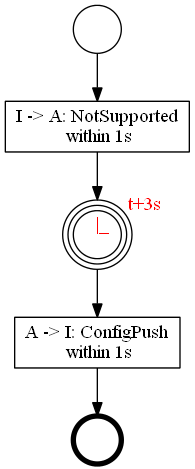
\includegraphics[height=6cm]{Delay}
\end{column}
\begin{column}<1->[b]{6cm}
\begin{exampleblock}<1->{}
{\BLUE global protocol} FirstDelay (role A, role I) \{ \\
~~NotSupported {\BLUE from} I {\BLUE to} A {\BLUE within} 1s;\\
~~{\BLUE wait for} t+ 3s\\
 ~~ConfigPush {\BLUE from} A {\BLUE to} I {\BLUE within} 1s;\\
\}\\
\end{exampleblock}
~~\\
~~\\
~~\\
~~\\
\end{column}
\end{columns}
\end{frame}

\begin{frame}{How to write grammar with ANTLR?}
\begin{columns}
\begin{column}<1->[b]{5cm}
\begin{exampleblock}<1->{}
{\BLUE choice at} U \{ \\
~~	PushMode(InstrumentId) {\BLUE from} U {\BLUE to} A;\\
\} {\BLUE or} \{ \\
~~	PollMode(InstrumentId,int) {\BLUE from} U {\BLUE to} A;\\
\}
\end{exampleblock}
\end{column}
\end{columns}
~~\\
~~\\
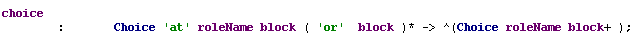
\includegraphics[width=11cm]{choicerule2}
~~\\
~~\\
~~\\
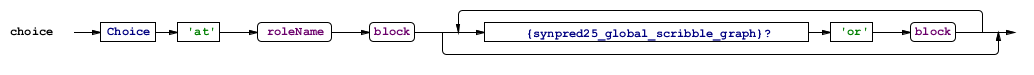
\includegraphics[width = 11.5cm]{choicerule}
\end{frame}

\begin{frame}{Class diagrams}
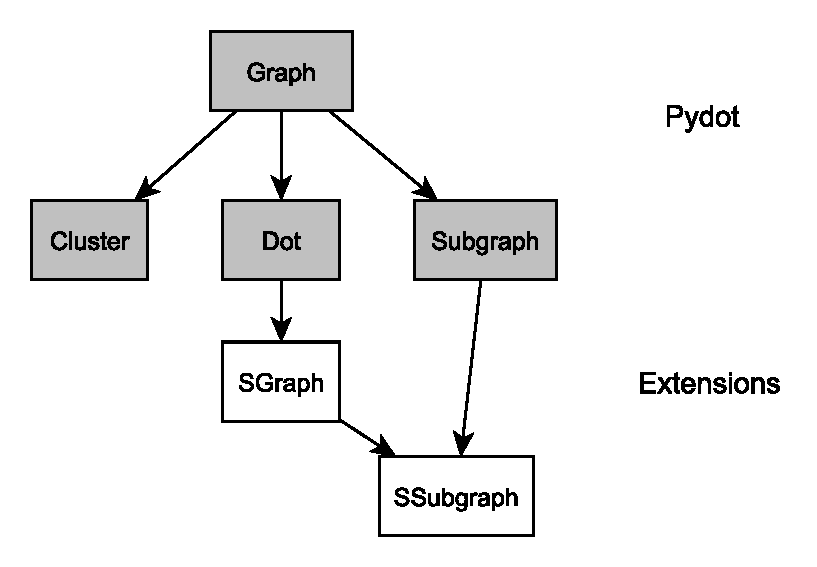
\includegraphics[scale=0.5]{graph_organisation}
~~\\
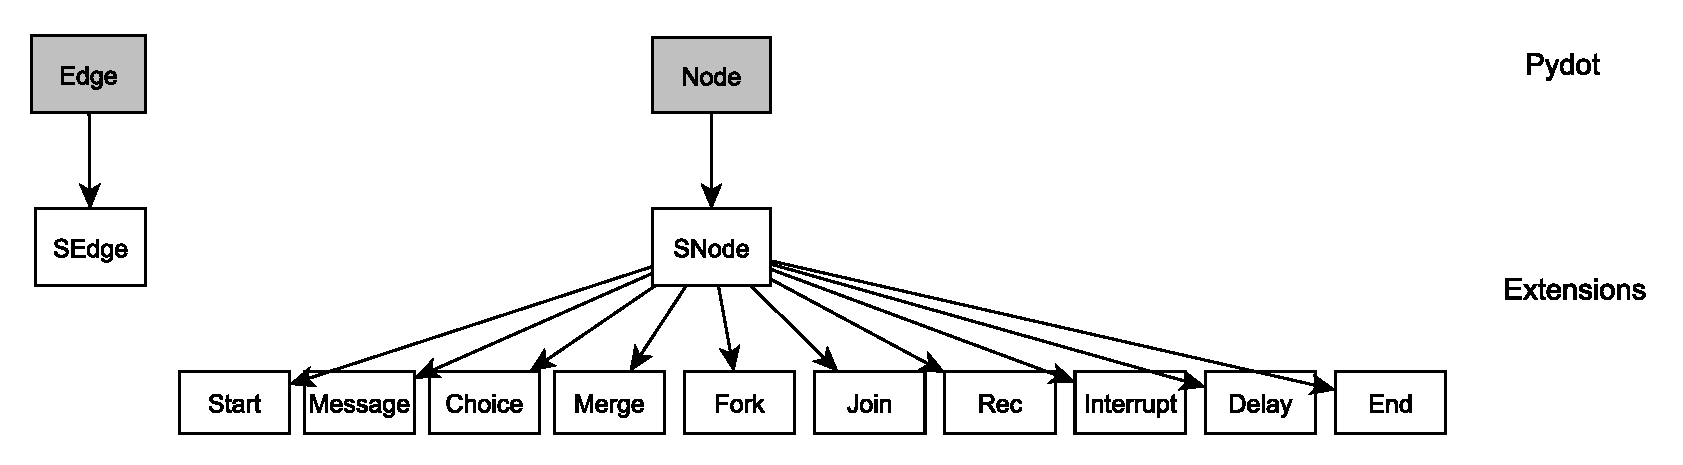
\includegraphics[width=11cm]{node_organisation}
\end{frame}

\end{document}

